% !TeX spellcheck = en_US
\documentclass[a4paper,12pt]{article}
\usepackage{listings}
%\usepackage[T1]{fontenc}
\usepackage{fontspec}
\usepackage[greek, english]{babel}
\usepackage[super]{nth}
\usepackage{fancyhdr}
\usepackage[left=1.50cm, right=1.50cm, top=2cm, bottom=1.cm, includeheadfoot]{geometry}
\usepackage{amsmath}
\usepackage{graphicx}
\usepackage{subcaption}
\usepackage{float}
%\usepackage[colorinlistoftodos]{todonotes}
\usepackage{xcolor}
\usepackage{ulem}
\usepackage{amsmath}
\usepackage{caption}
\usepackage{subcaption}
\usepackage{tabularray}
\usepackage[framed]{matlab-prettifier}
\usepackage{svg}
\usepackage{nth}
\usepackage{wrapfig}
\usepackage{siunitx}
\sisetup{output-exponent-marker=\ensuremath{\mathrm{e}}}
\usepackage{bm}

\usepackage[pdfauthor={Alexandra Gianni, Nikos Stylianou},
pdftitle={Second Problem Set},
pdfcreator={TeX},
pdfsubject={ECE447 - Neuro-Fuzzy Computing}]{hyperref}


\hypersetup{
	colorlinks,
	citecolor=blue,
	filecolor=black,
	linkcolor=black,
	urlcolor=blue
}

\lstset{
	style              = Matlab-editor,
	basicstyle         = \footnotesize,
	escapechar         = ",
	mlshowsectionrules = true,
}

\setmainfont{Times New Roman}

\pagestyle{fancy}
\fancyhf{}
\fancyhead[l]{\footnotesize \nth{2} Problem Set}
\fancyhead[r]{\footnotesize Neuro-Fuzzy Computing}
%\fancyfoot[r]{\footnotesize \thepage}
\renewcommand{\footrulewidth}{0.4pt} % Line at the footer visible

\fancyfoot[c]{\thepage}

\fancypagestyle{first}{
	\fancyhf{}
	\renewcommand{\headrulewidth}{0pt}
	\fancyfoot[c]{{\large \today}}
	\renewcommand{\footrulewidth}{0.0pt} % Line at the footer visible
} 

\newcommand{\MathSpace}{\ }
\setlength{\parindent}{0pt} % Paragraph identation is set to 0

\newcommand\ddfrac[2]{\frac{\displaystyle #1}{\displaystyle #2}} % Better fractions for inline

\renewcommand{\thesubsection}{(\alph{subsection})} % Change subsection style
\renewcommand{\thesection}{\hspace{-18pt}} % Make section style look nicer
\renewcommand\thesubsubsection{\thesection\hspace{18pt}(\alph{subsection}). \roman{subsubsection}}

\definecolor{veraman}{HTML}{55928A}

\begin{document}
	
	\begin{titlepage}
		\thispagestyle{first}
		
		\newcommand{\HRule}{\rule{\linewidth}{0.5mm}} % Defines a new command for the horizontal lines, change thickness here
		
		\center % Center everything on the page
		
		%----------------------------------------------------------------------------------------
		%	HEADING SECTIONS
		%----------------------------------------------------------------------------------------
		
		\textsc{\LARGE University of Thessaly}\\[1.6cm] % Name of your university/college
		
\includegraphics[scale=.5]{Images/uth-logo.png}\\[1cm] % Include a department/university logo - this will require the graphicx package
		\textsc{\Large Neuro-Fuzzy Computing}\\[0.6cm] % Major heading such as course name
		\textsc{\large ECE447}\\[0.5cm] % Minor heading such as course title
		
		%----------------------------------------------------------------------------------------
		%	TITLE SECTION
		%----------------------------------------------------------------------------------------
		
		\HRule \\[0.5cm]
		{ \huge \nth{2} Problem Set}\\[0.4cm] % Title of your document
		\HRule \\[1.8cm]
		
		%----------------------------------------------------------------------------------------
		%	AUTHOR SECTION
		%----------------------------------------------------------------------------------------
		
		
		\vspace*{1cm}
		\begin{minipage}{\textwidth}
			\centering
			\begin{tblr}{cc}
				 \emph{{\LARGE Alexandra Gianni}} & \emph{{\LARGE Nikos Stylianou}} \\ [3mm]
				 \emph{{\LARGE ID: 3382}} & \emph{{\LARGE ID: 2917}} \\
			\end{tblr}
		\end{minipage}\\[2.5cm]
		
		% If you don't want a supervisor, uncomment the two lines below and remove the section above
		%\Large \emph{Author:}\\
		%John \textsc{Smith}\\[3cm] % Your name
		
		%----------------------------------------------------------------------------------------
		%	DATE SECTION
		%----------------------------------------------------------------------------------------
		
		
		%\vfill % Fill the rest of the page with whitespace
		
	\end{titlepage}
	
	% !TeX spellcheck = en_US
\section{Problem 1}
In this exercise we need to find the minimum of the given 2-dimensional function:\\
\begin{equation}	
		F(\mathbf{w})=w_{1}^{2}+w_{2}^{2}+(0.5w_{1}+w_{2})^{2}+(0.5w_{1}+w_{2})^{4}
	\label{eq:function1}	
\end{equation}
with the Conjugate Gradient (Fletcher-Reeves) method and the Gradient Descent.\\

Initially, we can conclude that the function $F(w)$ is not in quadratic form because of the term $(0.5w_{1}+w_{2})^{4}$.
A function is said to be in quadratic form if it can be expressed as a second-degree polynomial where all the terms are either squared terms or cross-products of the variables. The presence of the fourth-degree term $(0.5w_{1}+w_{2})^{4}$.
makes this function a higher-degree polynomial, specifically a quartic function with respect to $(0.5w_{1}+w_{2})$, which means it cannot be classified as quadratic.\\
Also, the independent values in this function are $w_{1},w_{2}$, because only with them we can manipulate the $F(w)$.\\ 

As an initial guess we have $w\left(0\right) = \left[3, 3\right]^T$.\\
Τhe steps we have to use are specific for each iteration

\begin{center}
	\underline{\textit{FIRST ITERATION k = 0}}
\end{center}

\underline{Step1: Calculate the Gradient at  $w\left(k\right)$ }\\
\(\nabla f(w_1,w_2) = \left(\begin{array}{c}
	\dfrac{\partial f}{\partial w_1} \\[4mm]
	\dfrac{\partial f}{\partial w_2}
\end{array}\right)\) = $\left(\begin{array}{c}
	2w_1 + (0.5w_1+w_2) + 2(0.5w_1+w_2)^3\\[1mm]
	2w_2 + 2(0.5w_1+w_2) + 4(0.5w_1+w_2)^3
\end{array}\right) = \left(\begin{array}{c}
	2.5w_1 + w_2 + 2(0.5w_1+w_2)^3\\[1mm]
	w_1 + 4w_2 + 4(0.5w_1+w_2)^3
\end{array}\right)$ \\[3mm]

where at the point $w\left(0\right) = \left[3, 3\right]^T$ we have $\nabla f(x) = \left(\begin{array}{c}
	-53 \\
	-19
\end{array}\right)$
\\[4mm]

\begin{center}
	\underline{\textbf{GRADIENT DESCENT}}
\end{center}
Gradient descent is one of the most favored optimization technique, because of its simplicity and its generality.\\
In order to find the minimum of the Function ~\ref{eq:function1} we must first initialize our initial point $w_{0}$, value of tolerance $tol$ and Step size\\
Given the same initial guess $w\left(0\right) = \left[3, 3\right]^T$. \\
In order to find the minimum of the function~\ref{eq:function1} we need to follow the Gradient Descent's steps:\\

\underline{Step 1: Initialize initial point $w_{0}$, value of tolerance $tol$ and Step size}\\
As we have mentioned, the initial values are:
\begin{itemize}
	\item $w\left(0\right) = \left[3, 3\right]^T$
	\item $tol = 10^{-6}$
	\item $\alpha = 0.01$\\
	The exercise says that we apply the GD method with unit step movement. However, if we set $\alpha = 1$, which is considered a large value, the algorithm may not converge to the optimal point and it will even diverge completely. That's why we set $\alpha = 0.01$. 
\end{itemize} 
\vspace{2mm}

Taking these initializations into account, we follow the Gradient Descent's steps:\\

\underline{Step 1: Compute gradient $\nabla f$ at $w_{k}$}
\vspace{4mm}

\underline{Step 2: Make a scaled step in the opposite direction to the gradient}\\
\begin{equation}
	\begin{gathered}
		\text{step} = \alpha \cdot \nabla f_{k}\\
	\end{gathered}
\end{equation}
\vspace{2mm}

\underline{Step 3: Check convergence}\\
If the step size is smaller than the convergence, then we stop. Else, we repeat Step 1 and Step 2 while we update $x$.
\vspace{4mm}

\underline{Step 4: Update $x$}
\begin{equation}
	x_{k+1} = x_{k} - \alpha \cdot \nabla f_{k}
\end{equation}
\vspace{4mm}

Taking these steps into consideration we will attempt to minimize our function.\\

\begin{center}
	\underline{\textit{ITERATION k = 0}}
\end{center}

\underline{Step 1: Compute Gradient}\\
\(\nabla f(w_1,w_2) = \left(\begin{array}{c}
	\dfrac{\partial f}{\partial w_1} \\[4mm]
	\dfrac{\partial f}{\partial w_2}
\end{array}\right)\) = $\left(\begin{array}{c}
	2w_1 + (0.5w_1+w_2) + 2(0.5w_1+w_2)^3\\[1mm]
	2w_2 + 2(0.5w_1+w_2) + 4(0.5w_1+w_2)^3
\end{array}\right) = \left(\begin{array}{c}
	2.5w_1 + w_2 + 2(0.5w_1+w_2)^3\\[1mm]
	w_1 + 4w_2 + 4(0.5w_1+w_2)^3
\end{array}\right)$ \\[3mm]

where at the point $w\left(0\right) = \left[3, 3\right]^T$ we have $\nabla f_{0} = \left(\begin{array}{c}
	192.75 \\
	379.5
\end{array}\right)$
\\[4mm]

\underline{Step 2: Step size}
\[
step = a \cdot \nabla f_{0} = 0.01 \cdot \left(\begin{array}{c}
	192.75 \\
	379.5
\end{array}\right) \rightarrow step =\left(\begin{array}{c}
1.92750 \\
3.7950
\end{array}\right)
\]
\\[4mm]

\underline{Step 3: Check Convergence}\\
The norm of the step size is $\| step \| = 4.256440 > tol$, so we update $w$
\\[4mm]

\underline{Step 4: Update}
\[ 
w_1 = w_0 - a\cdot \nabla f_0 =  \left[\begin{array}{c}
	3 \\
	3
\end{array}\right] - \left(\begin{array}{c}
1.92750 \\
3.7950
\end{array}\right) \rightarrow
w_1 = \left[\begin{array}{c}
	 1.073\\
	 -0.795
\end{array}\right]
\]
\\[4mm]

\begin{center}
	\underline{\textit{ITERATION k = 1}}
\end{center}

\underline{Step 1: Compute Gradient}\\
\(\nabla f(w_1,w_2) = \left(\begin{array}{c}
	\dfrac{\partial f}{\partial w_1} \\[4mm]
	\dfrac{\partial f}{\partial w_2}
\end{array}\right)\) $= \left(\begin{array}{c}
	2.5w_1 + w_2 + 2(0.5w_1+w_2)^3\\[1mm]
	w_1 + 4w_2 + 4(0.5w_1+w_2)^3
\end{array}\right)$ \\[3mm]

where at the point $w\left(1\right) = \left[1.073, -0.795\right]^T$ we have $\nabla f_{1} = \left(\begin{array}{c}
	1.851603 \\
	-2.176795
\end{array}\right)$
\\[4mm]

\underline{Step 2: Step size}
\[
step = a \cdot \nabla f_{1} = 0.01 \cdot \left(\begin{array}{c}
1.851603 \\
-2.176795
\end{array}\right) \rightarrow step =\left(\begin{array}{c}
	0.018516 \\
	-0.021768
\end{array}\right)
\]
\\[4mm]

\underline{Step 3: Check Convergence}\\
The norm of the step size is $\| step \| = \num{2.857773e-02 }> tol$, so we update $w$
\\[4mm]

\underline{Step 4: Update}
\[ 
w_2 = w_1 - a\cdot \nabla f_1 =  \left[\begin{array}{c}
 1.073\\
-0.795
\end{array}\right] - \left(\begin{array}{c}
	0.018516 \\
	-0.021768
\end{array}\right) \rightarrow
w_2 = \left[\begin{array}{c}
	1.054\\
	-0.773
\end{array}\right]
\]
\\[4mm]

\begin{center}
	\underline{\textit{ITERATION k = 2}}
\end{center}

\underline{Step 1: Compute Gradient}\\
\(\nabla f(w_1,w_2) = \left(\begin{array}{c}
	\dfrac{\partial f}{\partial w_1} \\[4mm]
	\dfrac{\partial f}{\partial w_2}
\end{array}\right)\) $= \left(\begin{array}{c}
	2.5w_1 + w_2 + 2(0.5w_1+w_2)^3\\[1mm]
	w_1 + 4w_2 + 4(0.5w_1+w_2)^3
\end{array}\right)$ \\[3mm]

where at the point $w\left(2\right) = \left[1.054, -0.773\right]^T$ we have $\nabla f_{2} = \left(\begin{array}{c}
	1.831867 \\
	-2.098666
\end{array}\right)$
\\[4mm]

\underline{Step 2: Step size}
\[
step = a \cdot \nabla f_{2} = 0.01 \cdot \left(\begin{array}{c}
	1.831867 \\
   -2.098666
\end{array}\right) \rightarrow step =\left(\begin{array}{c}
	0.018319 \\
	-0.020987
\end{array}\right)
\]
\\[4mm]

\underline{Step 3: Check Convergence}\\
The norm of the step size is $\| step \| = \num{2.785702e-02} > tol$, so we update $w$
\\[4mm]

\underline{Step 4: Update}
\[ 
w_3 = w_2 - a\cdot \nabla f_2 =  \left[\begin{array}{c}
	1.054 \\
	-0.773
\end{array}\right] - \left(\begin{array}{c}
	0.018319 \\
-0.020987
\end{array}\right) \rightarrow
w_3 = \left[\begin{array}{c}
	1.036\\
	-0.752
\end{array}\right]
\]
\\[4mm]

\begin{center}
	\underline{\textit{ITERATION k = 3}}
\end{center}

\underline{Step 1: Compute Gradient}\\
\(\nabla f(w_1,w_2) = \left(\begin{array}{c}
	\dfrac{\partial f}{\partial w_1} \\[4mm]
	\dfrac{\partial f}{\partial w_2}
\end{array}\right)\) $= \left(\begin{array}{c}
	2.5w_1 + w_2 + 2(0.5w_1+w_2)^3\\[1mm]
	w_1 + 4w_2 + 4(0.5w_1+w_2)^3
\end{array}\right)$ \\[3mm]

where at the point $w\left(3\right) = \left[1.036, -0.752\right]^T$ we have $\nabla f_{3} = \left(\begin{array}{c}
	1.811156 \\
	-2.024840
\end{array}\right)$
\\[4mm]

\underline{Step 2: Step size}
\[
step = a \cdot \nabla f_{3} = 0.01 \cdot \left(\begin{array}{c}
	1.811156 \\
-2.024840
\end{array}\right) \rightarrow step =\left(\begin{array}{c}
	0.018112 \\
	-0.020248
\end{array}\right)
\]
\\[4mm]

\underline{Step 3: Check Convergence}\\
The norm of the step size is $\| step \| = \num{2.716664e-02} > tol$, so we update $w$
\\[4mm]

\underline{Step 4: Update}
\[ 
w_4 = w_3 - a\cdot \nabla f_3 =  \left[\begin{array}{c}
	1.036\\
	-0.752
\end{array}\right] - \left(\begin{array}{c}
	0.018319 \\
	-0.020987
\end{array}\right) \rightarrow
w_4 = \left[\begin{array}{c}
	1.018\\
	-0.732
\end{array}\right]
\]
\\[4mm]

\begin{center}
	\underline{\textit{ITERATION k = 4}}
\end{center}

\underline{Step 1: Compute Gradient}\\
\(\nabla f(w_1,w_2) = \left(\begin{array}{c}
	\dfrac{\partial f}{\partial w_1} \\[4mm]
	\dfrac{\partial f}{\partial w_2}
\end{array}\right)\) $= \left(\begin{array}{c}
	2.5w_1 + w_2 + 2(0.5w_1+w_2)^3\\[1mm]
	w_1 + 4w_2 + 4(0.5w_1+w_2)^3
\end{array}\right)$ \\[3mm]

where at the point $w\left(4\right) = \left[1.018, -0.732\right]^T$ we have $\nabla f_{4} = \left(\begin{array}{c}
	1.789642 \\
	-1.954924
\end{array}\right)$
\\[4mm]

\underline{Step 2: Step size}
\[
step = a \cdot \nabla f_{4} = 0.01 \cdot \left(\begin{array}{c}
	1.789642 \\
-1.954924
\end{array}\right) \rightarrow step =\left(\begin{array}{c}
	0.017896 \\
	-0.019549
\end{array}\right)
\]
\\[4mm]

\underline{Step 3: Check Convergence}\\
The norm of the step size is $\| step \| = \num{2.650386e-02} > tol$, so we update $w$
\\[4mm]

\underline{Step 4: Update}
\[ 
w_5 = w_4 - a\cdot \nabla f_4 =  \left[\begin{array}{c}
	1.018\\
	-0.732
\end{array}\right] - \left(\begin{array}{c}
	0.017896 \\
-0.019549
\end{array}\right) \rightarrow
w_5 = \left[\begin{array}{c}
	1.000\\
	-0.712
\end{array}\right]
\]
\\[4mm]

\begin{center}
	\underline{\textit{ITERATION k = 5}}
\end{center}

\underline{Step 1: Compute Gradient}\\
\(\nabla f(w_1,w_2) = \left(\begin{array}{c}
	\dfrac{\partial f}{\partial w_1} \\[4mm]
	\dfrac{\partial f}{\partial w_2}
\end{array}\right)\) $= \left(\begin{array}{c}
	2.5w_1 + w_2 + 2(0.5w_1+w_2)^3\\[1mm]
	w_1 + 4w_2 + 4(0.5w_1+w_2)^3
\end{array}\right)$ \\[3mm]

where at the point $w\left(5\right) = \left[1.000, -0.712\right]^T$ we have $\nabla f_{5} = \left(\begin{array}{c}
	1.767472 \\
	-1.888581
\end{array}\right)$
\\[4mm]

\underline{Step 2: Step size}
\[
step = a \cdot \nabla f_{5} = 0.01 \cdot \left(\begin{array}{c}
	1.767472 \\
-1.888581
\end{array}\right) \rightarrow step =\left(\begin{array}{c}
0.017675 \\
-0.018886
\end{array}\right)
\]
\\[4mm]

\underline{Step 3: Check Convergence}\\
The norm of the step size is $\| step \| = \num{2.586638e-02} > tol$, so we update $w$
\\[4mm]

\underline{Step 4: Update}
\[ 
w_6 = w_5 - a\cdot \nabla f_5 =  \left[\begin{array}{c}
	1.000\\
	-0.712
\end{array}\right] - \left(\begin{array}{c}
0.017675 \\
-0.018886
\end{array}\right) \rightarrow
w_6 = \left[\begin{array}{c}
	0.982\\
	-0.694
\end{array}\right]
\]
\\[4mm]

\begin{center}
	\underline{\textit{ITERATION k = 6}}
\end{center}

\underline{Step 1: Compute Gradient}\\
\(\nabla f(w_1,w_2) = \left(\begin{array}{c}
	\dfrac{\partial f}{\partial w_1} \\[4mm]
	\dfrac{\partial f}{\partial w_2}
\end{array}\right)\) $= \left(\begin{array}{c}
	2.5w_1 + w_2 + 2(0.5w_1+w_2)^3\\[1mm]
	w_1 + 4w_2 + 4(0.5w_1+w_2)^3
\end{array}\right)$ \\[3mm]

where at the point $w\left(5\right) = \left[1.000, -0.712\right]^T$ we have $\nabla f_{5} = \left(\begin{array}{c}
	1.767472 \\
	-1.888581
\end{array}\right)$
\\[4mm]

\underline{Step 2: Step size}
\[
step = a \cdot \nabla f_{5} = 0.01 \cdot \left(\begin{array}{c}
	1.767472 \\
	-1.888581
\end{array}\right) \rightarrow step =\left(\begin{array}{c}
	0.017675 \\
	-0.018886
\end{array}\right)
\]
\\[4mm]

\underline{Step 3: Check Convergence}\\
The norm of the step size is $\| step \| = \num{2.586638e-02} > tol$, so we update $w$
\\[4mm]

\underline{Step 4: Update}
\[ 
w_6 = w_5 - a\cdot \nabla f_5 =  \left[\begin{array}{c}
	1.000\\
	-0.712
\end{array}\right] - \left(\begin{array}{c}
	0.017675 \\
	-0.018886
\end{array}\right) \rightarrow
w_6 = \left[\begin{array}{c}
	0.982\\
	-0.694
\end{array}\right]
\]
\\[4mm]

\begin{center}
	\underline{\textit{ITERATION k = 7}}
\end{center}

\underline{Step 1: Compute Gradient}\\
\(\nabla f(w_1,w_2) = \left(\begin{array}{c}
	\dfrac{\partial f}{\partial w_1} \\[4mm]
	\dfrac{\partial f}{\partial w_2}
\end{array}\right)\) $= \left(\begin{array}{c}
	2.5w_1 + w_2 + 2(0.5w_1+w_2)^3\\[1mm]
	w_1 + 4w_2 + 4(0.5w_1+w_2)^3
\end{array}\right)$ \\[3mm]

where at the point $w\left(5\right) = \left[1.000, -0.712\right]^T$ we have $\nabla f_{5} = \left(\begin{array}{c}
	1.767472 \\
	-1.888581
\end{array}\right)$
\\[4mm]

\underline{Step 2: Step size}
\[
step = a \cdot \nabla f_{5} = 0.01 \cdot \left(\begin{array}{c}
	1.767472 \\
	-1.888581
\end{array}\right) \rightarrow step =\left(\begin{array}{c}
	0.017675 \\
	-0.018886
\end{array}\right)
\]
\\[4mm]

\underline{Step 3: Check Convergence}\\
The norm of the step size is $\| step \| = \num{2.586638e-02} > tol$, so we update $w$
\\[4mm]

\underline{Step 4: Update}
\[ 
w_6 = w_5 - a\cdot \nabla f_5 =  \left[\begin{array}{c}
	1.000\\
	-0.712
\end{array}\right] - \left(\begin{array}{c}
	0.017675 \\
	-0.018886
\end{array}\right) \rightarrow
w_6 = \left[\begin{array}{c}
	0.982\\
	-0.694
\end{array}\right]
\]
\\[4mm]








	% !TeX spellcheck = en_US
\section{Problem 2}
Second-order optimization methods are a class of algorithms used for finding the minimum or maximum of a function. These methods are characterized by their use of second-order derivatives, specifically the $Hessian \ \ matrix$, which contains the second partial derivatives of the function being optimized. The use of that method takes into account the curvature of the function.\\

One of the most well-known second-order methods is Newton's method. It updates the paarameters by moving in the direction of the inverse Hessian matrix applied to the gradient.\\

The update rule is given by:
\begin{equation}
	x_{k+1} = x_k - H^{-1}\nabla F(x_k)
\end{equation}
where
\begin{itemize}
	\item $x_k$ is the parameter vector at iteration $k$
	\item $\nabla F(x_k)$ is the gradient and
	\item $ H^{-1}$ is the inverse of the Hessian matrix at $x_k$
\end{itemize}
\vspace{2mm}
With that being said, we need to find the minimum of the function
\begin{equation}	
	F(\mathbf{w})=w_{1}^{2}+w_{2}^{2}+(0.5w_{1}+w_{2})^{2}+(0.5w_{1}+w_{2})^{4}	
	\label{eq:Equation2}
\end{equation}


using the Newton method and fixed step $\lambda = 1$, even though this is not a quadratic form.\\

To implement the code we followed the algorithm's basic steps:\\

\underline{Step 1}: Calculate gradient $\mathbf{\nabla F(x_k)}$ and Hessian matrix $\mathbf{\nabla^2F(x_k)}$ \\

\underline{Step 2}: If we have no-quadratic form, find and calculate Inversive Hessian Matrix $\mathbf{H^{-1}}$\\

\underline{Step 3}: Compute the minimizing direction $\mathbf{s_{k}}$\\
The formula for the minimizing direction $s_{k}$ is
\begin{equation}
	\begin{gathered}
		s_{k} = \left[-\nabla^2F(x_k)\right]^{-1} \cdot \nabla F(x_k)\\
		\text{or for simplicity}\\
		s_{k} = -H^{-1} \cdot \nabla F(x_k)
	\end{gathered}
\end{equation}

\underline{Step 4}: Minimize $\mathbf{F(x_{k} + \lambda_{k} \cdot s_{k})}$ to find optimal $\lambda_{k}$\\
There are two ways to do it
\begin{itemize}
	\item By $\dfrac{d f(x_k - \lambda_k [\nabla^2 f(x_k)]^{-1} \nabla f(x_k))}{d \lambda_k} = 0$ or
	\item By using a 1D optimization method
\end{itemize}
Keep in mind that if our equation is in quadratic form we always suppose that $\lambda = 1$.\\
On our exercise, even though Equation~\ref{eq:Equation2} is not on quadratic form, we suppose that $\lambda$ has a fixed value of 1.\\

\underline{Step 5:} Calculate the next point $\mathbf{x_{k+1}}$\\
Each time, to find the next point we calculate:
\begin{equation}
	x_{k+1} = x_{k} + \lambda_{k} \cdot s_{k}
\end{equation}

\underline{Step 6:} Check convergence criterion\\
A condition that determines when an iterative process should stop because it has reached a solution that is close enough to the exact solution. \\
Hence, we define the tolerance: $\epsilon = 10^{-6}$
\vspace{2mm}

Everything considered, we implement these steps into \textit{"Newton.m"} and we conclude into the fact that:\\
\begin{enumerate}
	\item The minimum of the function occurs at $1.0e-12*$ with $\mathbf{x_{k} = [0.1055; 0.2109]}$\\
	This is the point where the minimum of the function occurs. The numbers $0.1055$ and $0.2109$ are the $x1$ and $x2$ coordinates of the minimum point, respectively. The $1.0e-12*$ indicates that these numbers are in the order of $10^{-12}$, so the actual coordinates are extremely close to zero, as we want to.
	\item The number of iterations is: $\mathbf{8}$
\end{enumerate}

We can visualize these results with the help of the following plots.

\begin{figure}[H]
	\centering
	\begin{subfigure}{0.45\textwidth}
		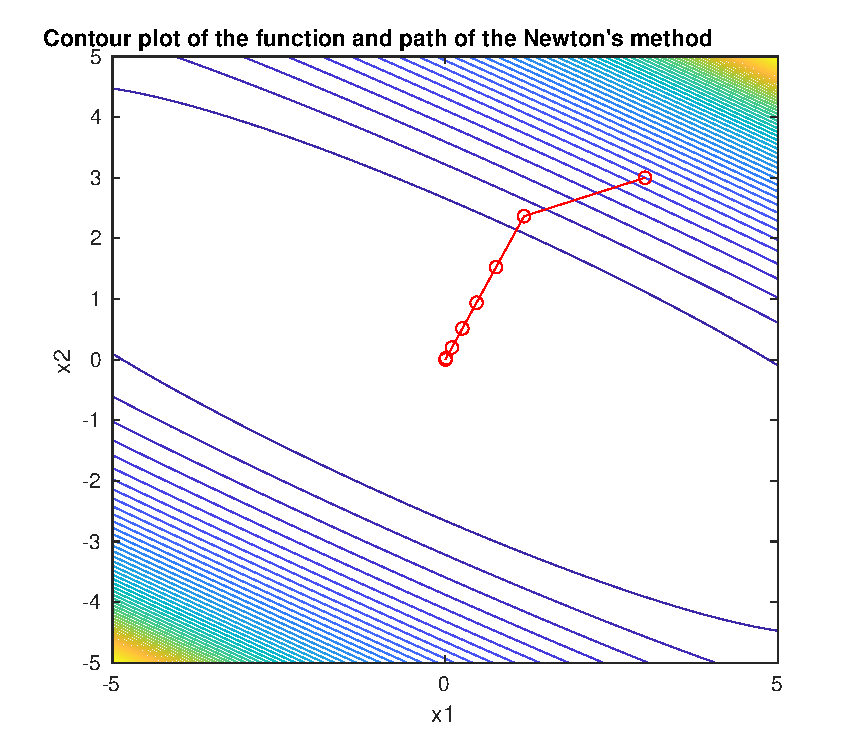
\includegraphics[width=\textwidth]{../Problem 2/contour_plot.pdf}
		\caption{Contour plot of the $F(w)$ function with path trajectory}
	\end{subfigure}
	\quad
	\begin{subfigure}{0.5\textwidth}
		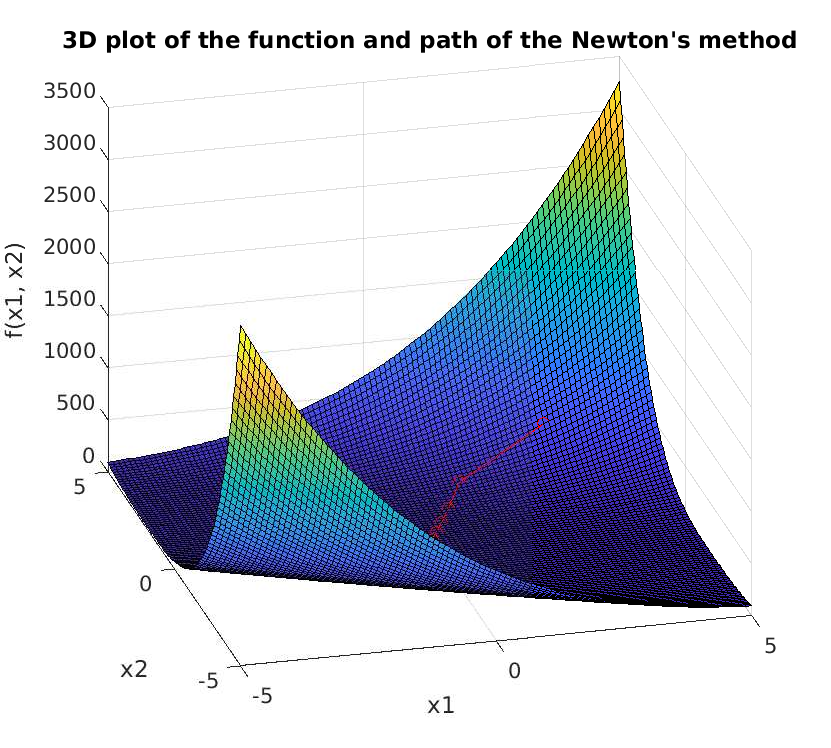
\includegraphics[width=\textwidth]{../Problem 2/3D_plot.pdf}
		\caption{3D visualization}
	\end{subfigure}
\end{figure}
\vspace{3mm}
The path represents the sequence of points visited by Newton's method as it converges to the minimum $[0; 0]$, highlighting the method's efficiency and directionality in navigating the function's terrain towards the optimum.\\

By comparing the Newton method with the previous ones, the Conjugate Gradient and the Gradient Descent method for solving optimization problems, several key differences and insights emerge:
\begin{enumerate}
	\item Convergence speed:\\
	The Newton method offers quadratic convergence under suitable conditions, which means it can converge to the solution in fewer iterations compared to CG and GD, especially when close to the optimum. However, this rapid convergence comes at the cost of calculating and inverting the Hessian matrix, which can be computationally expensive for high-dimensional problems.
	\item Computational complexity:\\
	Newton has high computational cost due to the necessity of computing and inverting the Hessian matrix at each iteration, in contrast with Conjugate gradient that does not require explicit computations for it. The Gradient Descent has the lowest computational cost per iteration among the three, as it only requires the calculation of the gradient. However, it may require more iterations to converge.
	\item Memory usage:\\
	The method that has the most requirements is the Newton method, because it requires more memory to store the Hessian matrix and its reverse. Next comes Conjugate gradient and at last Gradient Descent method has in general low memory requirements.
\end{enumerate}

In summary, we can conclude that the Gradient Descent method is the simplest algorithm among these three, the Conjugate gradient is more suitable for large-scale problems and the Newtons method is the fastest one. We understood that, because for the same function the one that converged first was the Newton's application. 




	% !TeX spellcheck = en_US
\section{Problem 3}

For the given neural network, we have:
\begin{itemize}
	\item learning rate $LR = 1$,
	\item $w^1\left(0\right) = -3,\ w^2\left(0\right) = -1$,
	\item $b^1\left(0\right) = 2,\ b^2\left(0\right) = -1$ and
	\item input/target pair $\left\{p=1,\ t=0\right\}$
\end{itemize}
\vspace*{1mm}

\begin{center}
	\underline{\textit{FIRST ITERATION}}
\end{center}

\underline{Step 1: Calculate first layer's output}
\[
\begin{gathered}
n^1 = w^1 p + b^1 = (-3)(1) + 2 = -1\\
a^1 = {Swish}\left(n^1\right) = {Swish}\left(-1\right) = \dfrac{n^1}{1+e^{-n^1}} = \dfrac{-1}{1+e} = -0.2689
\end{gathered}
\]

\underline{Step 2: Calculate second layer's output}
\[
\begin{gathered}
n^2 = w^2 a^1 + b^2 = (-1)(-0.2689) + (-1) = -0.7311 \\ 
a^2 = {LReLU}\left(n^2\right) = {LReLU}\left(-0.7311\right) = -0.000731
\end{gathered}
\]

\underline{Step 3: Calculate error}
\[
e = t-a^2 = \left(0-\left(-0.000731\right)\right) = 0.000731
\]

\underline{Step 4: Calculate sensitivity on second layer}
\[
s^2 = -2\ {LReLU}^{'}\left(n^2\right)\left(t-a^2\right) = -2 \left(0.001\right) \left(0.000731\right) = \num{-1.462e-06}
\]
\textit{\small LReLU's derivative is $1$ for $x>0$ and $0.001$ for $x<0$.}\\ 

\underline{Step 5: Calculate sensitivity on first layer using back-propagation}
\[
\begin{gathered}
s^1 = Swish^{'} \left(n^1\right) \left(w^2\right)^T s^2 = Swish^{'} \left(-1\right) \left(-1\right) (\num{-1.462e-06}) = 0.0723 (-1) (\num{-1.462e-06}) \\
s^1 = \num{1.0570e-07}
\end{gathered}
\]

\underline{Step 6: Update wheights and biases}
\[
\begin{gathered}
	w^{2}(1)=w^{2}(0)-LR\ s^{2}(a^{1})^{T} = -1 - 1(\num{-1.462e-06})(-0.2689) \approx -1 \\
	 b^{2}(1)=b^{2}(0)-LR\ s^{2} = -1 - 1(\num{-1.462e-06}) \approx -1 \\
	 w^{1}(1)=w^{1}(0)-LR\ s^{1}(a^{0})^{T} = -3 - 1(\num{1.0570e-07})(-1) \approx -3 \\
	 b^{1}(1)=b^{1}(0)-LR\ s^{1} = 2 - 1(\num{1.0570e-07}) \approx 2
\end{gathered}
\]

Since there were no changes on the biases and weights, the next iteration will not change the parameters of the given neural network, but we will calculate them anyway.
\vspace*{1mm}
\begin{center}
	\underline{\textit{SECOND ITERATION}}
\end{center}

\underline{Step 1:}
\[
\begin{gathered}
	n^1 = w^1 p + b^1 = (-3)(1) + 2 = -1\\
	a^1 = {Swish}\left(n^1\right) = {Swish}\left(-1\right) = \dfrac{n^1}{1+e^{-n^1}} = \dfrac{-1}{1+e} = -0.2689
\end{gathered}
\]

\underline{Step 2:}
\[
\begin{gathered}
	n^2 = w^2 a^1 + b^2 = (-1)(-0.2689) + (-1) = -0.7311 \\ 
	a^2 = {LReLU}\left(n^2\right) = {LReLU}\left(-0.7311\right) = -0.000731
\end{gathered}
\]

\underline{Step 3:}
\[
e = t-a^2 = \left(0-\left(-0.000731\right)\right) = 0.000731
\]

\underline{Step 4:}
\[
s^2 = -2\ {LReLU}^{'}\left(n^2\right)\left(t-a^2\right) = -2 \left(0.001\right) \left(0.000731\right) = \num{-1.462e-06}
\]

\underline{Step 5:}
\[
\begin{gathered}
	s^1 = Swish^{'} \left(n^1\right) \left(w^2\right)^T s^2 = Swish^{'} \left(-1\right) \left(-1\right) (\num{-1.462e-06}) = 0.0723 (-1) (\num{-1.462e-06}) \\
	s^1 = \num{1.0570e-07}
\end{gathered}
\]

\underline{Step 6:}
\[
\begin{gathered}
	w^{2}(1)=w^{2}(0)-LR\ s^{2}(a^{1})^{T} = -1 - 1(\num{-1.462e-06})(-0.2689) \approx -1 \\
	b^{2}(1)=b^{2}(0)-LR\ s^{2} = -1 - 1(\num{-1.462e-06}) \approx -1 \\
	w^{1}(1)=w^{1}(0)-LR\ s^{1}(a^{0})^{T} = -3 - 1(\num{1.0570e-07})(-1) \approx -3 \\
	b^{1}(1)=b^{1}(0)-LR\ s^{1} = 2 - 1(\num{1.0570e-07}) \approx 2
\end{gathered}
\]
	% !TeX spellcheck = en_US
\section{Problem 4}

In this problem, we are asked to write a program that implements backpropagation algorithm for an $1 - S^1 - 1$ network with $S^1=\left\{2,8,12\right\}$, as shown in figure~\ref{fig:prob4_nns}.

The first layer has $logsig$ as activation function and the output layer has $ReLU$ as activation function. Also, every weight and bias is initialized to a uniformly random number in $\left(-0.5, 0.5\right)$.
All of the above are done in order to train our network to approximate the following function:
\[
g(p) = 1 + e^{p\left(\dfrac{3\pi}{8}\right)}, \qquad p \in \left[-2,2\right]
\]

This means that, during training, we have to train the network for multiple input data (\textit{specifically, for all input data}).

\begin{figure}[H]
	\centering
	\begin{subfigure}{0.47\textwidth}
		\centering
		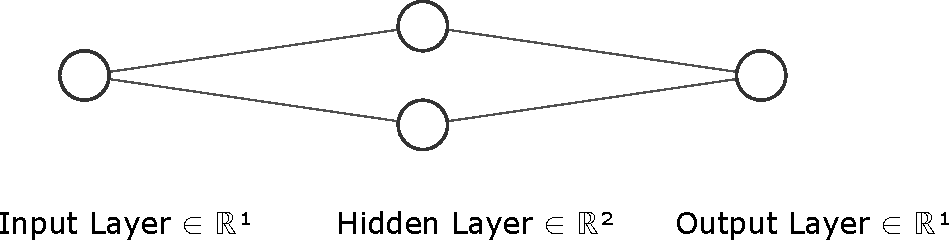
\includegraphics[width=0.9\textwidth]{../Problem 4/nn_1_2_1.pdf}
		\caption{$S^1=2$}
	\end{subfigure}
	\begin{subfigure}{0.47\textwidth}
		\centering
		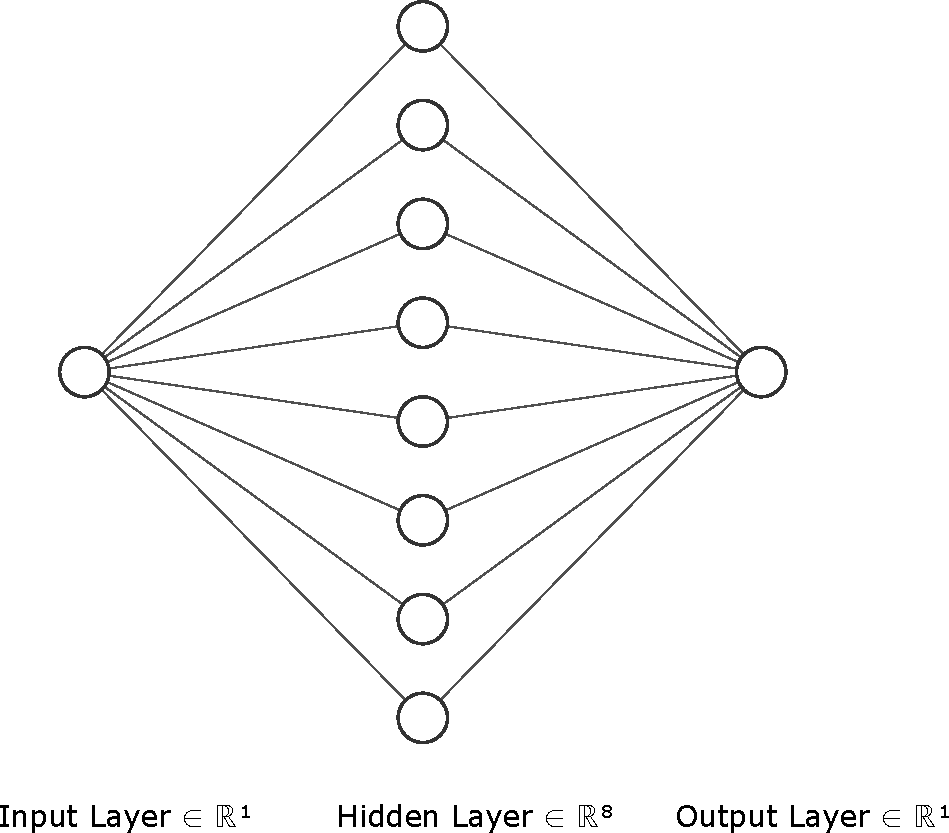
\includegraphics[width=0.9\textwidth]{../Problem 4/nn_1_8_1.pdf}
		\caption{$S^1=8$}
	\end{subfigure}
	\begin{subfigure}{0.47\textwidth}
		\centering
		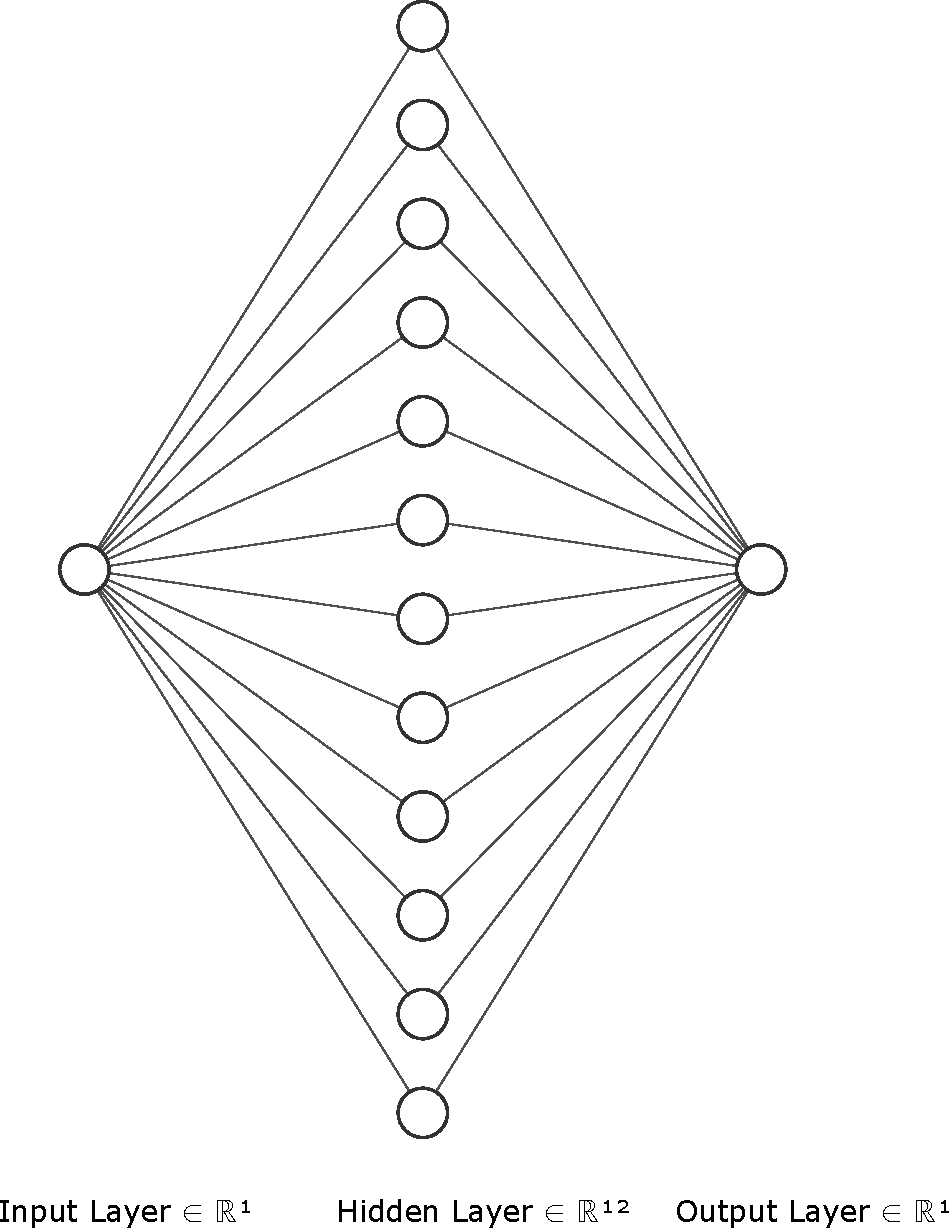
\includegraphics[width=\textwidth]{../Problem 4/nn_1_12_1.pdf}
		\caption{$S^1=12$}
	\end{subfigure}
	\caption{All the neural networks in this problem.}
	\label{fig:prob4_nns}
\end{figure}

We chose to write this program in MATLAB, despite the majority of these problems being written in Python. This ensures that we are going to use matrix operations for initialization of all weights and biases, as the problem .
The file \say{\textit{backpropagation.m}} contains all of the necessary code.\\

In order to see what difference $S$ and learning rate does to our network, we defined the following learning rates $\left[0.1, 0.01, 0.03, 0.001\right]$ and generated the network's output and error throughout training.

%From the first view, we can see in figure~\ref{fig:prob4_1_2_1_failed_attempt} that 
From the very first run ($S=2,\ \alpha=0.001$), we can see in figure~\ref{fig:prob4_1_2_1_failed_attempt} that the back-propagation algorithm didn't converge at all, keeping the error to a constant value throughout the epochs.

\begin{figure}[htpb]
	\centering
	\begin{subfigure}{0.47\textwidth}
		\centering
		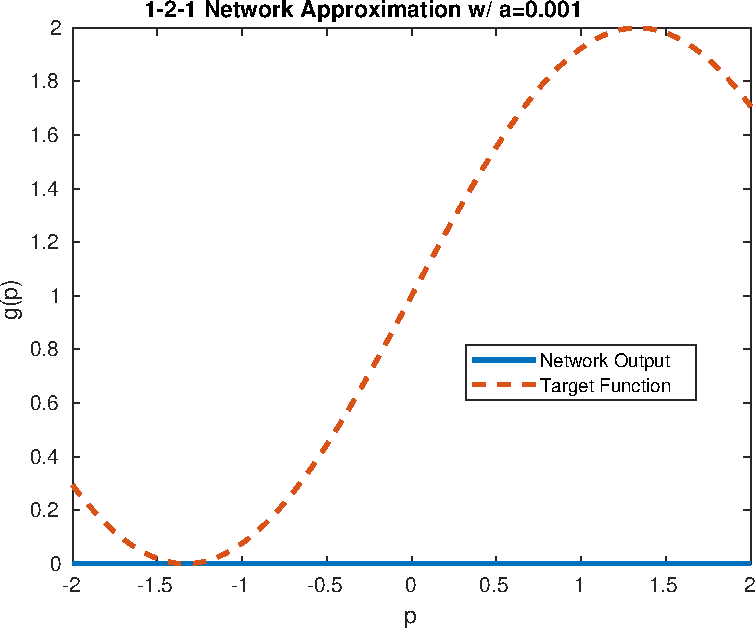
\includegraphics[width=\textwidth]{../Problem 4/1_2_1_failed_approximation.pdf}
		\caption{Approximation of input signal}
	\end{subfigure}
	\begin{subfigure}{0.47\textwidth}
		\centering
		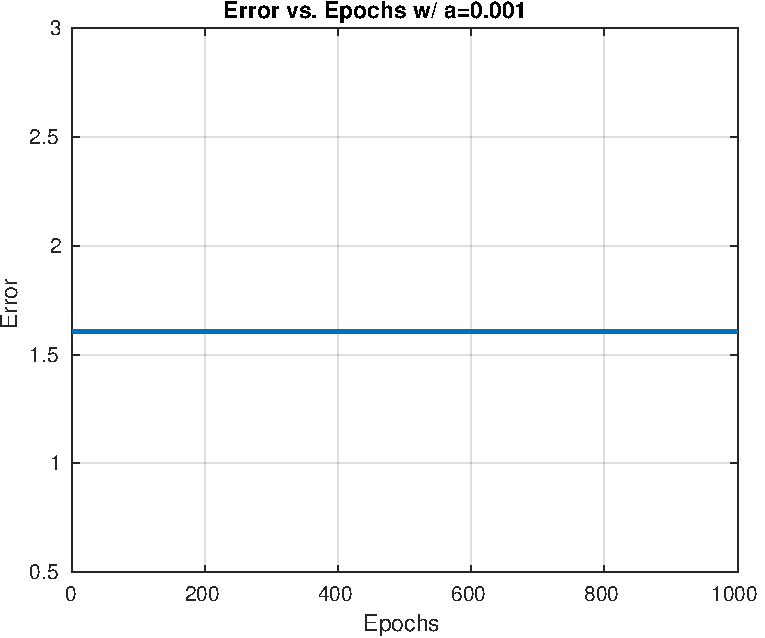
\includegraphics[width=\textwidth]{../Problem 4/1_2_1_failed_approximation_error.pdf}
		\caption{Error over iterations}
	\end{subfigure}
	\caption{A failed attempt of approximating the input signal. \\ The reason this approximation failed derives from the uniformly random initial guess for the weights and biases.}
	\label{fig:prob4_1_2_1_failed_attempt}
\end{figure}

After taking a closer look in the code, we can see the point of failure of the algorithm. Below, there's a snippet of the code that calculates the back-propagation.

\begin{lstlisting}[language=matlab]
	e = g(i) - a2;
	s2 = -2*e*relu_derivative(n2);
	s1 = logsig_derivative(n1) .* W2' .* s2;
\end{lstlisting}

We can see that both sensitivities depends on \verb*|s2|, a value that itself depends on $ReLU$'s derivative, which has the following expression:
\[
\dfrac{d\ ReLU\left(x\right)}{dx} = \left\{ 
\begin{array}{cc}
	1, & x >0\\
	0, & x<0
\end{array}
\right.
\]

So, if $n^2$ is a negative number, $ReLU$'s derivative will be $0$, zeroing out both sensitivities and effectively stalling the back-propagation algorithm. Thus, in order for the algorithm to make progress, $n^2$ \underline{must} be a positive number.
So, we altered the code and added an if statement that stops the algorithm if variable \verb*|s2=0| and \verb*|epoch=1|. In this way, we stop unnecessary calculations and start over, hopping that the random initialization of the weights and biases will not give us another configuration like the one above. \\

After describing the unexpected issue and its solution, we can focus on the real matter which is the accuracy of the algorithm across different learning rates and number of neurons in the first hidden layer. Figures~\ref{fig:prob4_1-2-1_error_output}, \ref{fig:prob4_1-8-1_error_output} and \ref{fig:prob4_1-12-1_error_output} contains every figure for every $S^1$ and learning rate $\alpha$.

\begin{figure}[htpb]
	\centering
	\begin{subfigure}{0.47\textwidth}
		\centering
		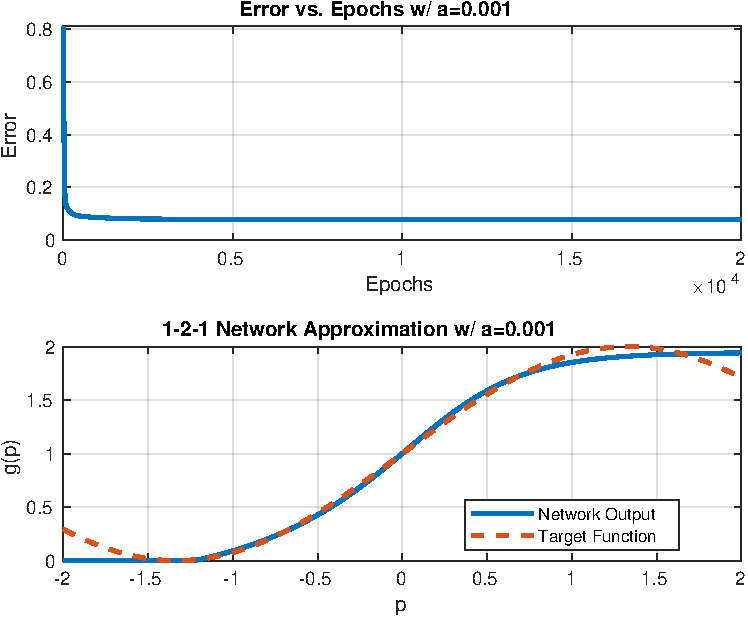
\includegraphics[width=\textwidth]{../Problem 4/nn_images/1-2-1_NN_a=0.001.pdf}
		\caption{}
	\end{subfigure}
	\hfill
	\begin{subfigure}{0.47\textwidth}
		\centering
		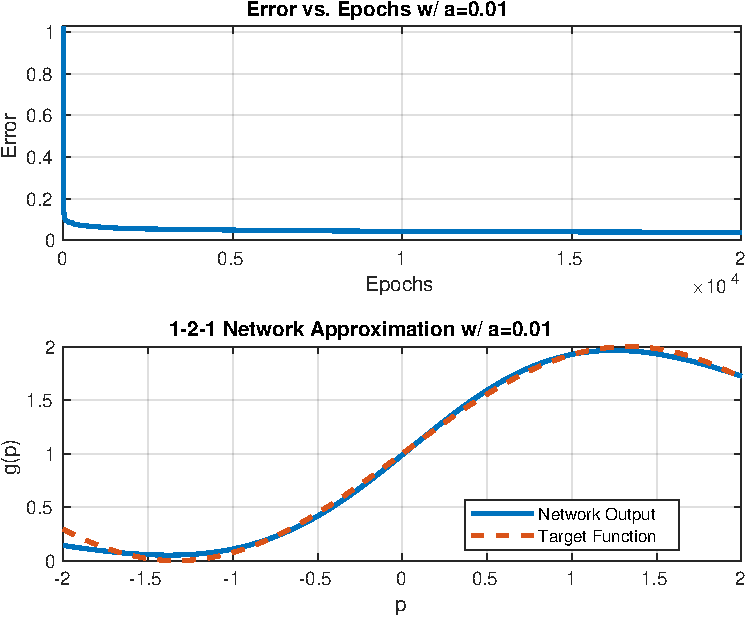
\includegraphics[width=\textwidth]{../Problem 4/nn_images/1-2-1_NN_a=0.01.pdf}
		\caption{}
	\end{subfigure}\\
	\vspace{1cm}
	\begin{subfigure}{0.47\textwidth}
		\centering
		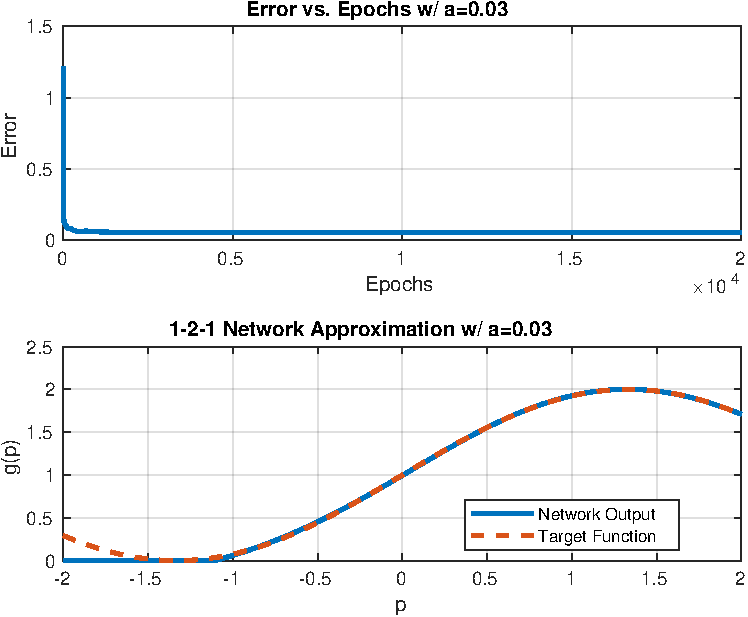
\includegraphics[width=\textwidth]{../Problem 4/nn_images/1-2-1_NN_a=0.03.pdf}
		\caption{}
	\end{subfigure}
	\hfill
	\begin{subfigure}{0.47\textwidth}
		\centering
		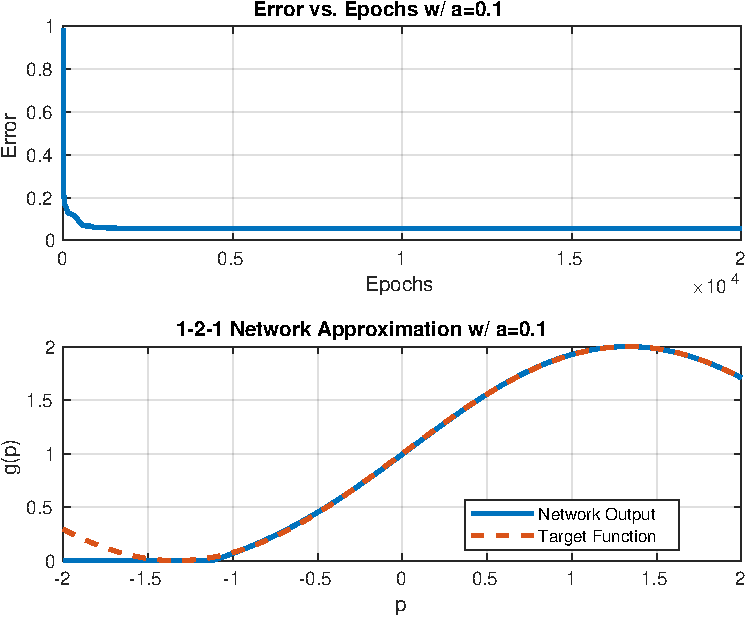
\includegraphics[width=\textwidth]{../Problem 4/nn_images/1-2-1_NN_a=0.1.pdf}
		\caption{}
	\end{subfigure}
	\caption{Error over iterations and approximation, $S^1=2$}
	\label{fig:prob4_1-2-1_error_output}
\end{figure}

\begin{figure}[htpb]
	\centering
	\begin{subfigure}{0.47\textwidth}
		\centering
		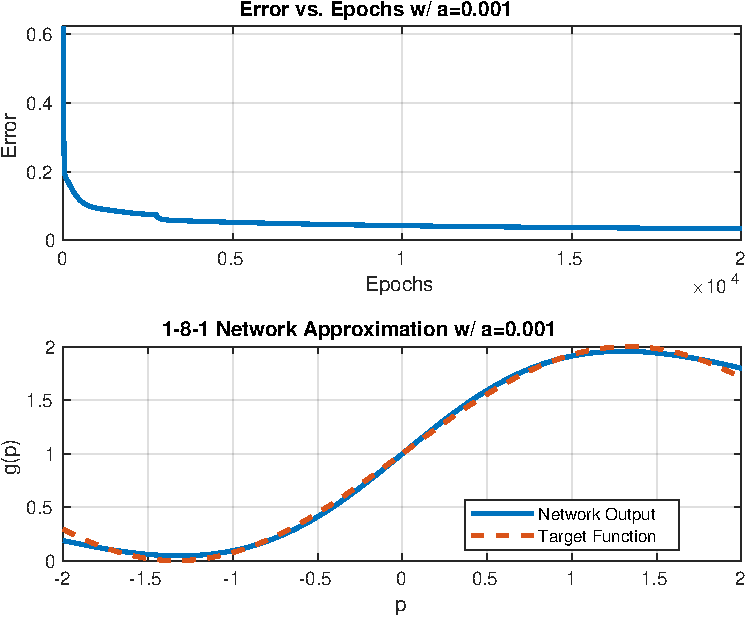
\includegraphics[width=\textwidth]{../Problem 4/nn_images/1-8-1_NN_a=0.001.pdf}
		\caption{}
	\end{subfigure}
	\hfill
	\begin{subfigure}{0.47\textwidth}
		\centering
		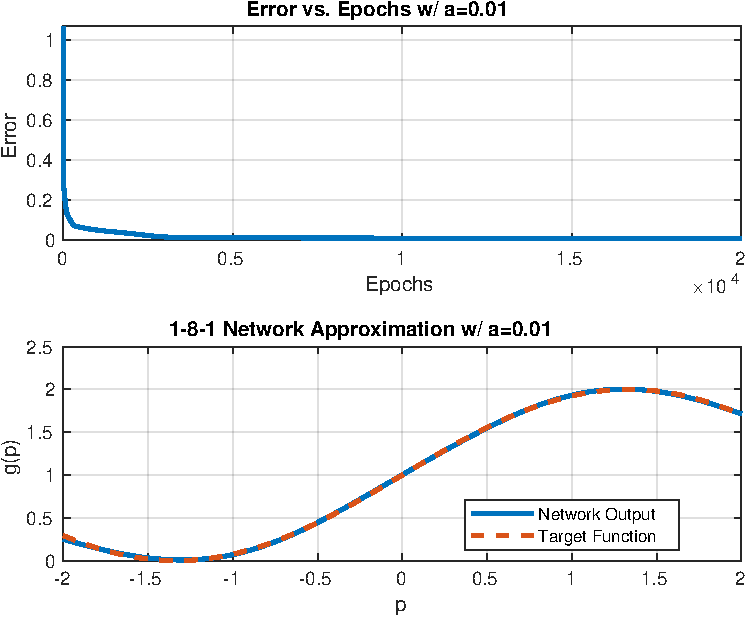
\includegraphics[width=\textwidth]{../Problem 4/nn_images/1-8-1_NN_a=0.01.pdf}
		\caption{}
	\end{subfigure}\\
	\vspace{1cm}
	\begin{subfigure}{0.47\textwidth}
		\centering
		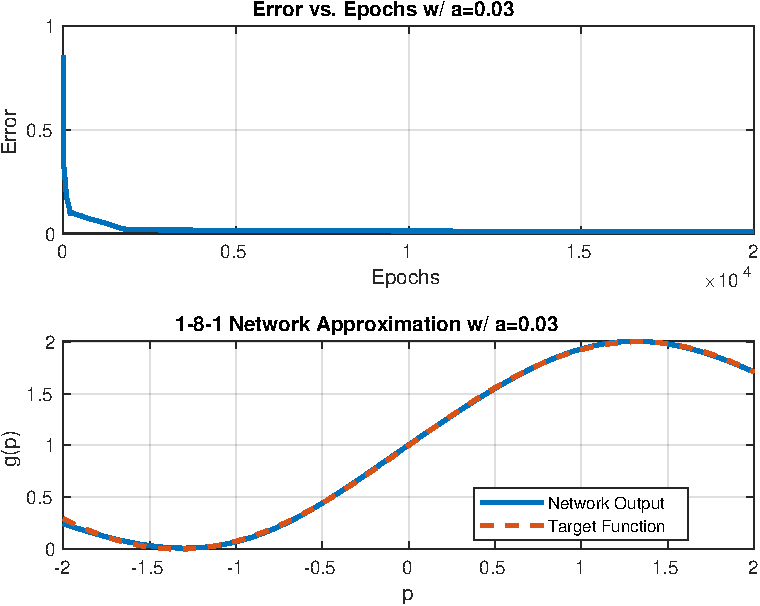
\includegraphics[width=\textwidth]{../Problem 4/nn_images/1-8-1_NN_a=0.03.pdf}
		\caption{}
	\end{subfigure}
	\hfill
	\begin{subfigure}{0.47\textwidth}
		\centering
		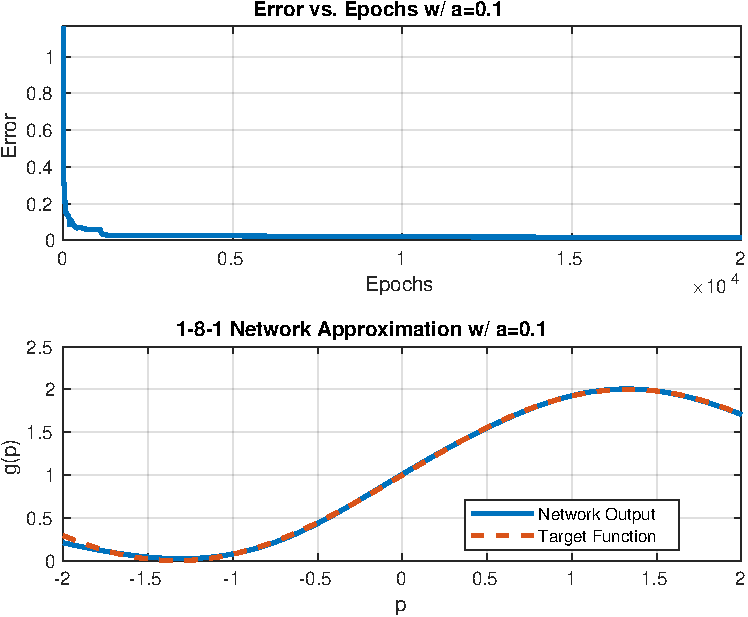
\includegraphics[width=\textwidth]{../Problem 4/nn_images/1-8-1_NN_a=0.1.pdf}
		\caption{}
	\end{subfigure}
	\caption{Error over iterations and approximation, $S^1=8$}
	\label{fig:prob4_1-8-1_error_output}
\end{figure}

\begin{figure}[htpb]
	\centering
	\begin{subfigure}{0.47\textwidth}
		\centering
		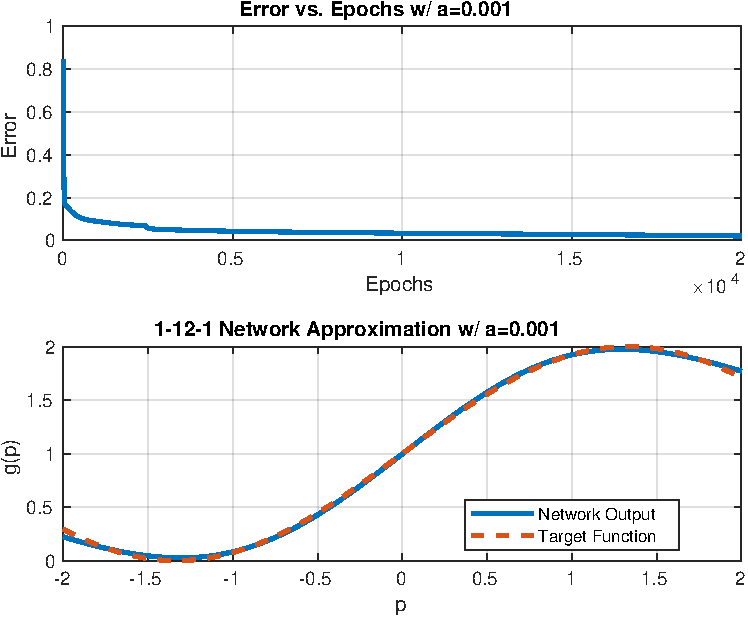
\includegraphics[width=\textwidth]{../Problem 4/nn_images/1-12-1_NN_a=0.001.pdf}
		\caption{}
	\end{subfigure}
	\hfill
	\begin{subfigure}{0.47\textwidth}
		\centering
		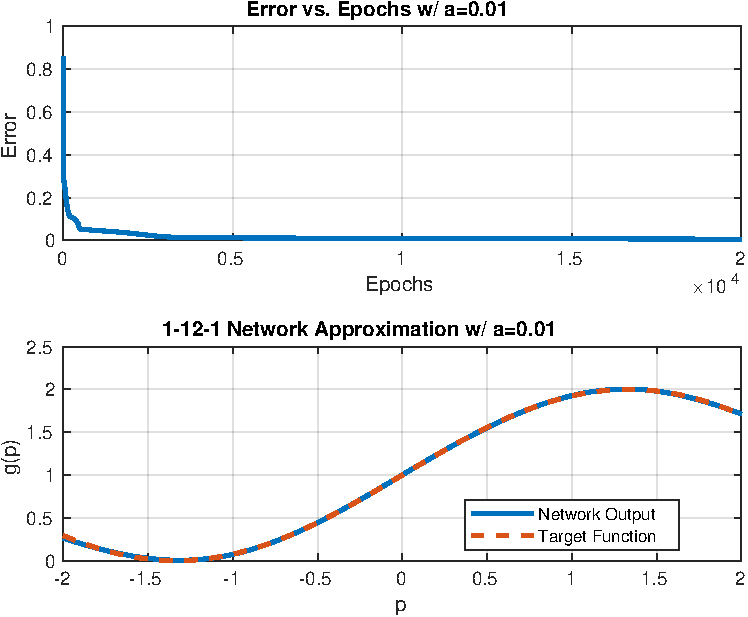
\includegraphics[width=\textwidth]{../Problem 4/nn_images/1-12-1_NN_a=0.01.pdf}
		\caption{}
	\end{subfigure}\\
	\vspace{1cm}
	\begin{subfigure}{0.47\textwidth}
		\centering
		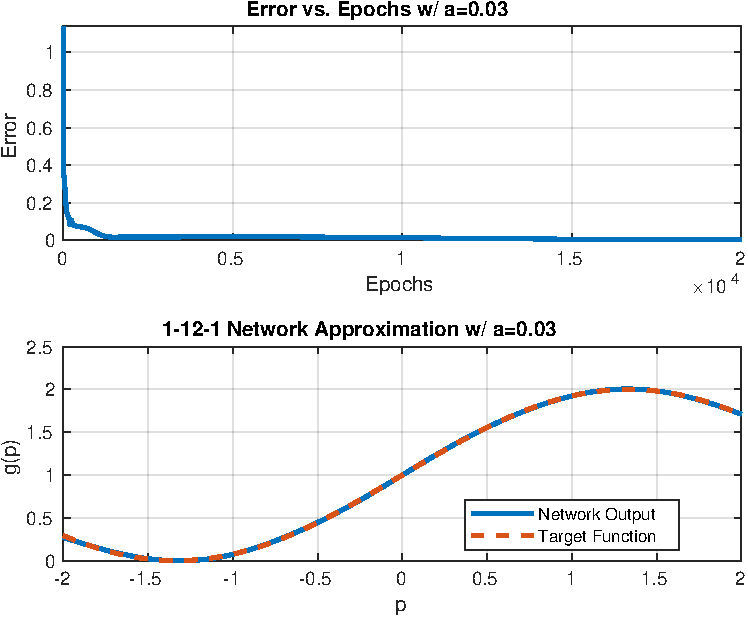
\includegraphics[width=\textwidth]{../Problem 4/nn_images/1-12-1_NN_a=0.03.pdf}
		\caption{}
	\end{subfigure}
	\hfill
	\begin{subfigure}{0.47\textwidth}
		\centering
		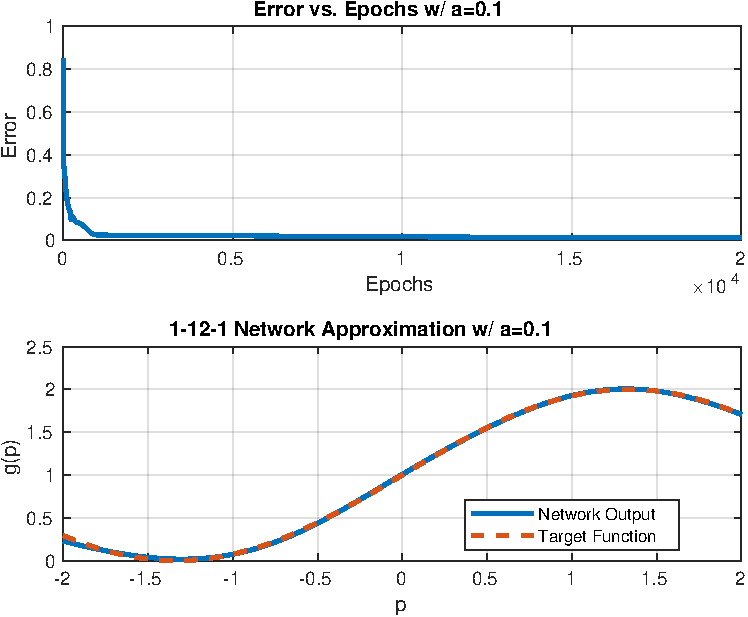
\includegraphics[width=\textwidth]{../Problem 4/nn_images/1-12-1_NN_a=0.1.pdf}
		\caption{}
	\end{subfigure}
	\caption{Error over iterations and approximation, $S^1=12$}
	\label{fig:prob4_1-12-1_error_output}
\end{figure}

The error plotted in every figure is the mean square approximation error described below:
\begin{lstlisting}[language=matlab]
	err = abs(a2_error' - g).^2;
	err_plt(epoch) = sqrt(mean(err));
\end{lstlisting}

As far as the learning rate $\alpha$ is concerned, we can observe that decreasing $\alpha$ results in a smoother but slower convergence. This indicates a more stable learning but requires a lot more iterations to achieve optimal accuracy.
On the other hand, higher $\alpha$ speed up convergence initially, but the end result is not great when comparing to smaller $\alpha$ values. Looking at the approximated functions, we can see that for $\alpha=0.1$ (\textit{\small which is a relatively big value}) there's a big approximation error for every $S^1$, thus accuracy is compromised.

We tried increasing $\alpha$ beyond $0.1$ but as it turned out, the algorithm failed each time either from the start or later. Regardless, we couldn't get any remarkable results for the report.\\

Moving on to the capacity of the hidden layer, there's a big change in the accuracy of the neural network as it's increased.
Looking at figure~\ref{fig:prob4_1-2-1_error_output}, we can see that there's a fairly large area at the start and end of $p$, where the approximation is way off the input signal.
As $S^1$ increases, the function's approximation on the areas described above is getting smaller as seen in figures~\ref{fig:prob4_1-8-1_error_output} and \ref{fig:prob4_1-12-1_error_output}. Particularly, in the latter the error drops very low for $\alpha=0.03$ and the approximation is almost the same as the original signal.
Also, this can be seen in the \say{Error vs Epochs} plot where the error drops very low. \\


In conclusion, our experiments reveal a subtle relationship between the learning rate, $\alpha$, and the capacity of the neural network, as defined by the number of hidden neurons, $S^1$. A lower $\alpha$ ensures stable and smooth convergence, albeit at the cost of increased iterations for optimal accuracy. Conversely, a higher $\alpha$ expedites convergence but at the expense of accuracy, particularly evident at $\alpha=0.1$ where the approximation error significantly increases across all $S^1$ values. Furthermore, our attempts to increase $\alpha$ beyond 0.1 resulted in algorithmic failure, underscoring the delicate balance required in tuning $\alpha$. On the capacity front, enhancing $S^1$ markedly improves the neural network's accuracy, particularly for complex function approximations as the neural network can process much more information. This is demonstrated through improved approximation closeness to the original signal with increased $S^1$, highlighting the critical role of neural network capacity in achieving high-fidelity approximations.
	% !TeX spellcheck = en_US
\section{Problem 5}
	% !TeX spellcheck = en_US
\section{Problem 7}
A continuous piecewise linear function is a function that is linear on every segment of its domain.\\
To show that a Multi-Layer Perceptron (MLP) using only the ReLU (Rectified Linear Unit) or pReLU (Parametric Rectified Linear Unit) activation functions constructs a continuous linear function, we must first review the properties of these activation functions. \\

Let’s consider the ReLU activation function for this explanation.

The ReLU activation function is defined as:\\
\begin{equation}
	\operatorname{ReLU}(x)=\operatorname*{max}(x,0)={\left\{\begin{array}{ll}
			{x}&{{\mathrm{if~}}x>0,}\\ 
			{0}&{{\mathrm{otherwise,}}}
			\end{array}\right.}		
\end{equation}

We need to check if they meet the prerequisites of continuity and linearity.
\begin{itemize}
	\item \underline{Is it Continuous?}\\
	Yes it is, because it has no break points for the various values of $x$
	\item \underline{Is it Linear?}\\
	Yes it is, because it consists of only two linear parts. ReLU is linear within its segments.
\end{itemize}

In an MLP, the output of each neuron is computed by applying an affine transformation (multiplying the weights and adding the bias), followed by ReLU activation. The key property of ReLU activation is that it is a piecewise linear function.
When you consider a single neuron with ReLU activation, it essentially performs two operations:
\begin{enumerate}
	\item For inputs $x$ where $x > 0$, the output is $x$.
	\item For inputs $x$ where $x \leq 0$, the output is $0$
\end{enumerate}

Having a closer look, the first operation $(x > 0)$ is a linear transformation with a slope of $1$ (output is $y = x$), and the second operation $(x \leq 0)$ is a constant zero (output is $y = 0$).\\

By composing several such neurons in an MLP architecture, we effectively create a composition of linear transformations and constant zeros. Since the operations of the individual ReLU neurons are piecewise linear, the combination of these operations is naturally also a piecewise linear function.\\
The breakpoints in the piecewise linear function occur where the activations of the neurons go from $0$ to the actual linear operation -when the input $x$ exceeds $0$ -. As you move from one layer to the next in the network, we are effectively combining multiple piecewise linear functions, resulting in a more complex piecewise linear function overall.\\

The activation function pReLU behaves similarly, but it introduces a learnable parameter $a$ for the negative slope that allows a continuous range of slopes for the linear part when $x$ is negative.\\

To summarize, an MLP that uses only ReLU (or pReLU) activation functions constructs a continuous piecewise linear function because the operations performed by these activation functions are individually piecewise linear and the composition of these operations across the layers results in a piecewise linear function that approximates complex mappings between inputs and outputs.\\

We can see also the graphical explaination  here:
\begin{figure}[h]
	\centering
	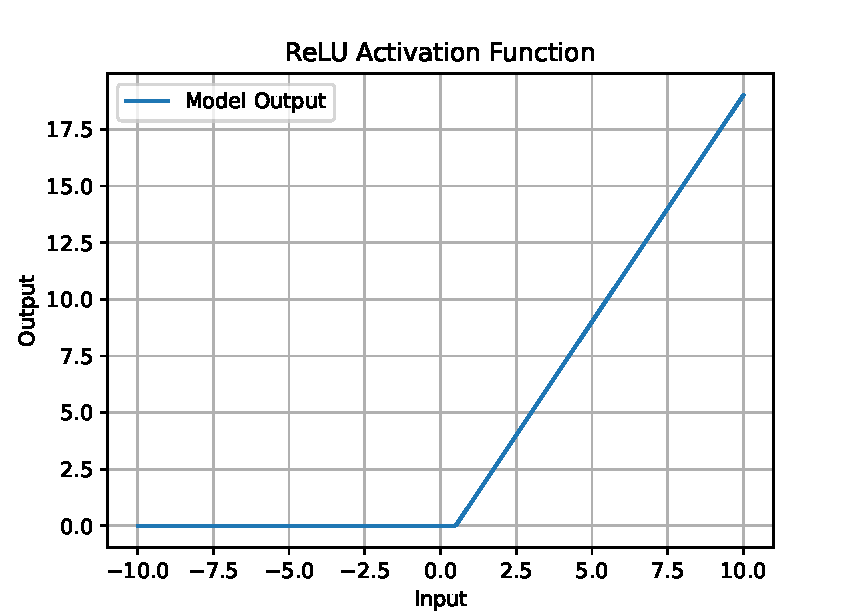
\includegraphics[width=0.6\textwidth]{../Problem 7/MLP_ReLU_plot.pdf}
	\caption{Plot of the MLP using the ReLU activation function}
\end{figure}
\vspace{5mm}


 


<<<<<<< Updated upstream
	% !TeX spellcheck = en_US
\section{Problem 10}

We are given the following update rule:
\begin{equation}
\begin{array}{l}{{g_{t+1}\ \leftarrow\beta\cdot g_{t}+(1-\beta)\cdot\nabla \hat{L}_{t}(\theta_{t})}}\\ {{\theta_{t+1}\ \leftarrow\theta_{t}-\alpha\left[(1-\nu)\cdot\nabla\hat{L}_{t}(\theta_{t})+\nu\cdot g_{t+1}\right]}}\end{array}
\label{eq:qhm_equation}
\end{equation}
, where $\alpha,\ \beta, \nu \in \Re$ and $\alpha$ is the learning rate.
$\hat{L}_{t}\left(\theta_{t}\right)$ represents a loss function which is minimized via $\theta$.\\

When examining the equation, we start to see a relation with SGD, but with some extra elements on the equation.
If we set $\mathbf{\left(\beta, \nu\right) = \left(0,1\right)}$ in order to eliminate some of the elements, we get the following expression:

\[
\left\{
\begin{array}{l}
	g_{t+1} \leftarrow \nabla \hat{L}_{t}\left(\theta_{t}\right)\\
	\theta_{t+1}\leftarrow\theta_{t}-\alpha \cdot g_{t+1}
\end{array}
\right\} \ =\  \theta_{t+1} \leftarrow \theta_{t} - \alpha \nabla \hat{L}_{t} \left(\theta_{t}\right)
\]
\vspace{1mm}

\underline{This is exactly the update rule of SGD} (\textit{Stochastic Gradient Descent}) found in our lectures, parameterized by $\alpha$.
We can get the SGD's update rule with one more pair of $\left(\beta, \nu  \right)$ values. By setting $\mathbf{\left(\beta, \nu\right) = \left(0,0\right)}$, we effectively eliminate term $g_{t+1}$. So, we get:
\[
\theta_{t+1}\leftarrow\theta_{t}-\alpha\cdot\nabla\hat{L}_{t}(\theta_{t})
\]
which is again the update rule for SGD.

Another form of the famous SGD is SGD with momentum, and has the following update rule:
\[
\begin{array}{l}
	{{g_{t+1}\leftarrow\beta\cdot g_{t}+(1-\beta) \cdot \nabla \hat{L}_{t}(\theta_{t})}}\\ {{\theta_{t+1}\leftarrow\theta_{t}-\alpha\cdot g_{t+1}}}
	\end{array}
\]
\\
SGD with momentum is an extension of the basic stochastic gradient descent algorithm, designed to accelerate learning, especially in the context of high curvature, small but consistent gradients, or noisy gradients. \\
In this extension, instead of using only the gradient of the current step to guide the learning process, we also take into account the gradient of the previous steps. This is typically done by keeping a running average of the gradients.\\

By looking the equation~\ref{eq:qhm_equation}, \underline{we can clearly obtain the update rule of SGD with momentum} easily. We just need to remove the term $\left(1 -\nu \right) \cdot \nabla \hat{L}_{t}\left(\theta_{t}\right)$ from $\theta_{t+1}$ and we will get the update rule of SGD with momentum.
This term is zeroed only when $\nu = 1$ and term $\beta$ is necessary in the update rule, thus a pair of values $\mathbf{\left(\beta, \nu\right) = \left(\beta, 1\right)}$.\\

Nesterov's accelerated gradient, that we've seen in our lectures, is another enhancement of \textit{GD} that \say{looks ahead} in the direction of the gradient. It's update rule is:
\[
\begin{array}{l}
	g_{t+1} \leftarrow \beta \cdot g_t + \left(1 - \beta \right) \cdot \nabla \hat{L}_t \left(\theta_t\right) \\ 
	\theta_{t+1} \leftarrow \theta_{t} - \alpha \cdot g_{t+1}
\end{array}
\]

If we observe the update rule from above, we can see that the whole term after $\alpha$ in $\theta_{t+1}$'s update rule is set to $g_{t+1}$. So, we only need to equal those two terms. This is a relatively easy task, as all we have to do is to set $\nu = \beta$ in equation~\ref{eq:qhm_equation}. By doing this replacement, we get:
\[
\left\{
\begin{array}{l}
	g_{t+1} \leftarrow \beta \cdot g_t + \left(1-\beta\right) \cdot \nabla \hat{L}_t \left(\theta_{t}\right) \\ 
	\theta_{t+1} \leftarrow \theta_{t} - \alpha \left[ \left(1-\beta\right) \cdot \nabla \hat{L}_t \left(\theta_{t}\right) + \beta \cdot g_{t+1} \right]
\end{array}
\right\} \Rightarrow
\left\{
\begin{array}{l}
	g_{t+1} \leftarrow \beta \cdot g_t + \left(1-\beta\right) \cdot \nabla \hat{L}_t \left(\theta_{t}\right) \\ 
	\theta_{t+1} \leftarrow \theta_{t} - \alpha \cdot g_{t+1}
\end{array}
\right\}
\]
Thus, we also extracted Nesterov's GD with success.\\

Unfortunately, we cannot extract any other familiar optimization method because they introduce sums and other complex operations in the update rule but the given method does not contain any of those. This formula represents a single, unified optimization method that \underline{is a variation of SGD} with momentum, rather than multiple distinct methods that can be extracted.

=======
	% !TeX spellcheck = en_US
\section{Problem 8}
Adadelta is another variant of the AdaGrad algorithm. The main difference lies in the fact that it decreases the amount by which the learning rate is adaptive to coordinates. Moreover, traditionally it referred to as not having a learning rate since it uses the amount of change itself as calibration for future change. Adadelta is an extension to the Gradient Descent Optimization Algorithm. Although, it is better understood as an extension of the AdaGrad and RMSProp algorithms. \\

The idea was derived mainly from ADAGRAD in order to improve upon the two main drawbacks of the method.
\begin{enumerate}
	\item The continual decay of learning rates throughout training
	\item The need for a manually selected
	global learning rate
\end{enumerate}

All things considered, in this exercise we are given the following function:
\begin{equation}
	F(w) = 0.1w_1^2 + 2w_2^2
\end{equation}
\label{eq:Funcproblem8}
\vspace{1mm}

\subsection{Question A}
To find the minimum of the Function ~\ref{eq:Funcproblem8} using the AdaDelta optimizer, instead of the gradient descent, we need to iteratively update the weights $w_1$ and $w_2$ based on the optimizer's rules. ADADELTA is an adaptive learning rate optimization algorithm that adjust the learning rate during training.\\

The Adadelta algorithm has two main parameters: $\rho$ and $e$. We will set:
\begin{itemize}
	\item Decay rate $\rho = 0.9$
	\item Constant $\epsilon = 10^{-6}$ 
\end{itemize}

$\epsilon$ is a small value which is added to maintain numerical stability.\\
The $\rho$ variable is a hyperparameter that controls the decay rate of the running averages of the squared gradients, $\mathbf{s}_{t}$, and squared parameter updates,	$\Delta{\bf x}_{t}$.\\

Based on these values, we will briefly explain the algorithm of AdaDelta. In a nutshell, AdaDelta uses two state variables, $\bm{s_t}$ to store a leaky average of the second moment of the gradient and $\bm{\Delta x_t$} to store a leaky average of the second moment of the change of parameters in the model itself.\\

Given the parameter $\rho$, we obtain the following leaky updates:
\begin{equation}
	\mathbf{s}_{t}=\rho\mathbf{s}_{t-1}+(1-\rho)\mathbf{g}_{t}^{2}
\end{equation} 
A crucial point and difference from the RMSProp algorithm is that we perform updates with the rescaled gradient $\bm{g_t'}$. So, each time the weights are updated as:
\begin{equation}
	\mathbf{w}_{t}=\mathbf{w}_{t-1}-\mathbf{g}_{t}^{\prime}.
\end{equation}

where the rescaled gradient is calculated as:
\begin{equation}
	\mathbf{g}_{t}^{\prime}={\frac{\sqrt{\Delta\mathbf{x}_{t-1}+\epsilon}}{\sqrt{\mathbf{s}_{t}+\epsilon}}}~\mathbf{g}_{t}
\end{equation}

Here, $\bm{\Delta x_{t-1}}$ is the leaky average of the squared rescaled gradient $\mathbf{g}_{t}^{\prime}$. We initialize $\bm{\Delta x_{0} = 0}$ and update each step with ${g}_{t}^{\prime}$ as this equation shows:

\begin{equation}
	\Delta{\bf x}_{t}=\rho\Delta{\bf x}_{t-1}+(1-\rho){\bf g}_{t}^{\prime2},
\end{equation}

For a better understanding of the topic, we will provide a pseudo-code of the ADADELTA algorithm.
	\begin{algorithm}[H]
		\caption{Computing ADADELTA update at time $t$}
		\begin{algorithmic}
			\Require Decay rate $\rho$, Constant $\epsilon$, Learning rate $\alpha$
			\Require Initial parameter $x_1$
			\State Initialize accumulation variables $S_t\_0 = 0$, $\Delta x_t\_0 = 0$
			\For{$t = 1$ \textbf{to} $T$} 
			\State Compute Gradient: $g_t$
			\State Accumulate Gradient: $S_t = \rho S_{t-1} + (1 - \rho)g_t^2$
			\State Compute Update: $	\mathbf{g}_{t}^{\prime}={\frac{\sqrt{\Delta\mathbf{x}_{t-1}+\epsilon}}{\sqrt{\mathbf{s}_{t}+\epsilon}}}~\mathbf{g}_{t}$
			\State Accumulate Updates: 	$\Delta{\bf x}_{t}=\rho\Delta{\bf x}_{t-1}+(1-\rho){\bf g}_{t}^{\prime2}$
			\State Apply Update: $x_{t+1} = x_t - (a*g_{t}^{\prime})$
			\EndFor
		\end{algorithmic}
	\end{algorithm}
it is very important to emphasize on the tricky part of the provided pseudo-code, because we have slightly changed it. For this exercise we want to include the learning rate in our optimizer. However, as we mentioned before, AdaDelta is an optimizer that doesn't use a learning rate. Taking everything into account, we modified the traditional update
\begin{equation}
	{x}_{t+1}={x}_{t}-{g}_{t}^{\prime}.
\end{equation}
into
\begin{equation}
	x_{t+1} = x_t - (a \cdot g_{t}^{\prime})
\end{equation}

To conclude, to point out the operation of the AdaDelta algorithm, we will plot the algorithm’s trajectory on a contour plot of F(x) for \textit{number of iterations = $300$}.
\begin{figure}[H]
	\centering
	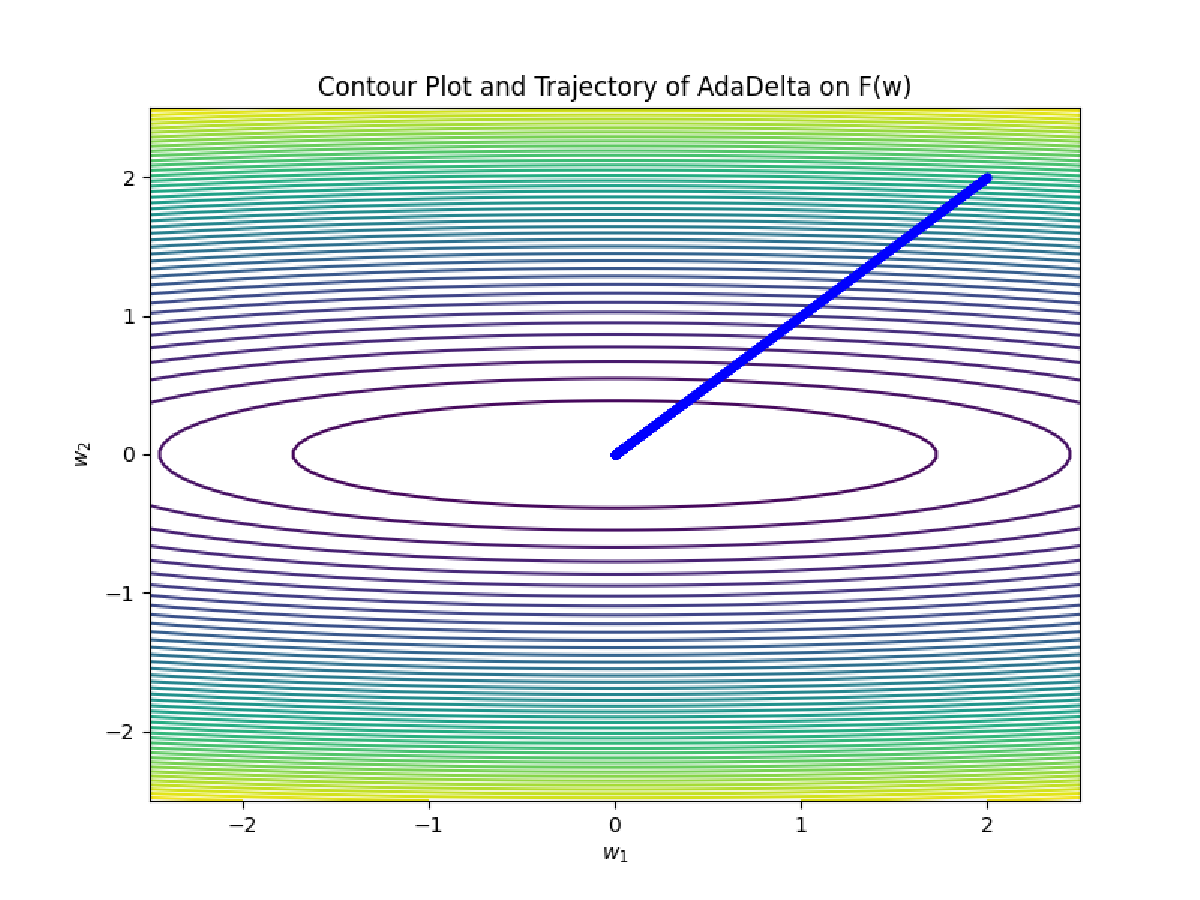
\includegraphics[width=.7\textwidth]{../Problem 8/ADADELTA_04.pdf}
	\caption{AdaDelta algorithm and trajectory with learning rate $\alpha=0.4$}
	\label{fig:lr=0.4}
\end{figure}
\vspace{2mm}

\subsection{Question B}
As previously mentioned, in the AdaDelta optimization algorithm, the learning rate is adaptively changed based on the running average of the recent gradients and the recent parameter updates. This is different from many other optimization algorithms where the learning rate is a fixed hyperparameter.\\
But, in this example we will show once again how by implementing some tricks we can still define it and observe how it can affect the algorithm's trajectory.\\

On the previous question, we plotted the algorithm's trajectory for learning rate $\alpha=0.4$. When we change it to $\alpha=3$ we can remark some crucial points.
\begin{figure}[H]
	\centering
	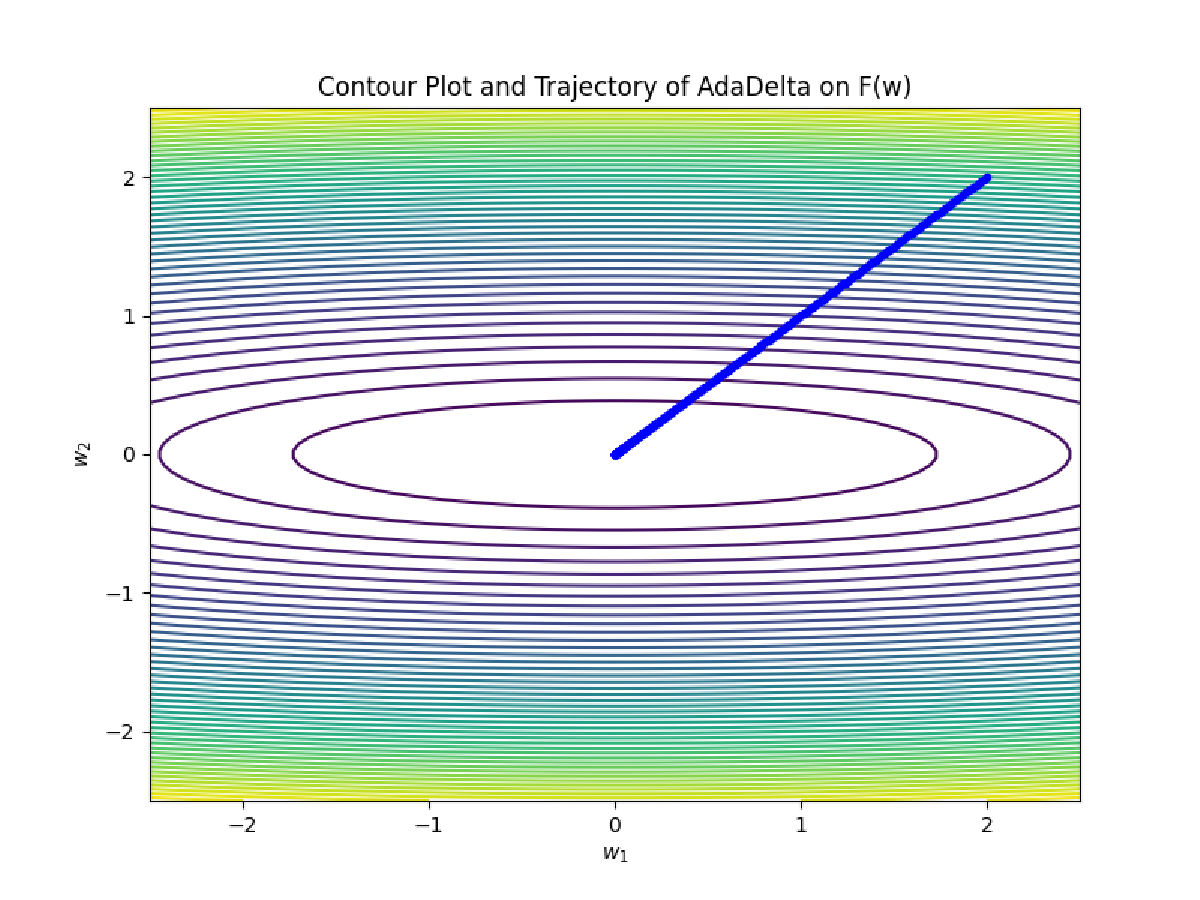
\includegraphics[width=.7\textwidth]{../Problem 8/ADADELTA_3.pdf}
	\caption{AdaDelta algorithm and trajectory with learning rate $\alpha=3$}
	\label{fig:lr=3}
\end{figure}
\vspace{2mm}

In drawing things to a close, based on Figure~\ref{fig:lr=0.4} and Figure~\ref{fig:lr=3} we can evaluate the impact of the learning rate and to take a closer look on the algorithm.\\

In both plots, the contours represent levels of the function $F(w)$ with each line indicating the points where the function has the same value. The closer the lines, the steeper the gradient at that point. The central region where the lines are more widely spaced indicates the minimum of the function.\\

The observation that we can highlight is the speed of convergence. A larger learning rate generally means that the optimizer makes larger steps in the parameter space. If the learning rate is set appropriately, this can lead to faster convergence to the minimum of the function. Though, there is a big risk of overshooting the minimum, which means that the optimizer could oscillate around the minimum, or in the worst case, to diverge.\\
Dissimilar to it, in Figure~\ref{fig:lr=3}, it appears that the AdaDelta optimizer with a higher learning rate has discovered a trajectory that approaches the function's central minimum more closely. This suggests that effective parameter space exploration has been made possible by the higher learning rate without leading to instability in the optimization procedure. With the same number of iteration, we accomplished the best convergence with a higher learning rate.
\vspace{2mm}

\subsection{Question C}


>>>>>>> Stashed changes
	% !TeX spellcheck = en_US
\section{Problem 11}
Convolutional Neural Networks (CNNs) have revolutionized in the field of image processing and computer vision and are widely utilized.\\

In this exercise we are considering a $6 x 6$ image I, where each entry represents the intensity of a pixel.The values are typically normalized , and the CNN would perform operations on this matrix to learn features and perform tasks like classification, detection, or segmentation. We will apply various layers and filters, so that we can extract higher-level features.\\


\begin{equation}
	I = \begin{bmatrix}
		20 & 35 & 35 & 35 & 35 & 20 \\
		29 & 46 & 44 & 42 & 42 & 27 \\
		16 & 25 & 21 & 19 & 19 & 12 \\
		66 & 120 & 116 & 154 & 114 & 62 \\
		74 & 216 & 174 & 252 & 172 & 112 \\
		70 & 210 & 170 & 250 & 170 & 110 \\
	\end{bmatrix}
	\label{tab:input_image}
\end{equation}
\vspace{2mm}

Given the input matrix we can understand that it represents a grayscale image. In a grayscale image, each pixel is represented by a single intensity value, typically on a scale $\left[0, 255\right]$. The 2D input array contains such intensity values for each pixel in the image.

\subsection{Question A}
The output of a convolution layer is a new matrix that's the result of the convolution operation. The convolution operation involves sliding the kernel over the input matrix, with a given stride $\left(1,1\right)$, and for each position, computing the sum of elementwise multiplications. \\

The use of a stride in a convolutional layer is important, because it determines how much the filter or kernel moves across the input matrix. In our case, a stride of $\left(1,1\right)$ means that the kernel moves one step at a time horizontally and vertically. This will result in an output matrix that is smaller than the input matrix by one less than the kernel size in each dimension. So, in our case the output will be a $4 x 4$. Also,the output's matrix size is smaller than the original because of the "valid" mode on our code. The "valid" mode means that the convolution product is only given for points where the kernels overlap completely with the input array. It doesn't add any padding to the input image.\\

In addition, the kernel we have defined is a $3 x 3$ matrix with a zero in the center. This means that the convolution operation will sum up the values of the eight surrounding pixels and ignore the center pixel for each position in the input image.\\

So, in conclusion, with a
\begin{itemize}
	\item $stride = \left(1,1\right)$ and 
	\item $	kernel = \begin{bmatrix}
		1 & 1 & 1  \\
		1 & 0 & 1  \\
		1 & 1 & 1  \\
	\end{bmatrix}$
\end{itemize}

The result of the convolution is a $ 4 x 4$ matrix\\

\begin{equation}
	result = \begin{bmatrix}
		225 & 258 & 250 & 209  \\
		458 & 566 & 552 & 472  \\
		708 & 981 & 887 & 802  \\
		1000 & 1488 & 1320 &1224 \\
	\end{bmatrix}
\end{equation}
\vspace{6mm}

The resulting matrix, represents the features in the input image that the kernel was able to detect. In this case, the kernel seems to act like a filter that emphasizes the surrounding context of each pixel. The exact interpretation would depend on the specific values in the input image and the kernel. 

\begin{figure}[h]
	\centering
	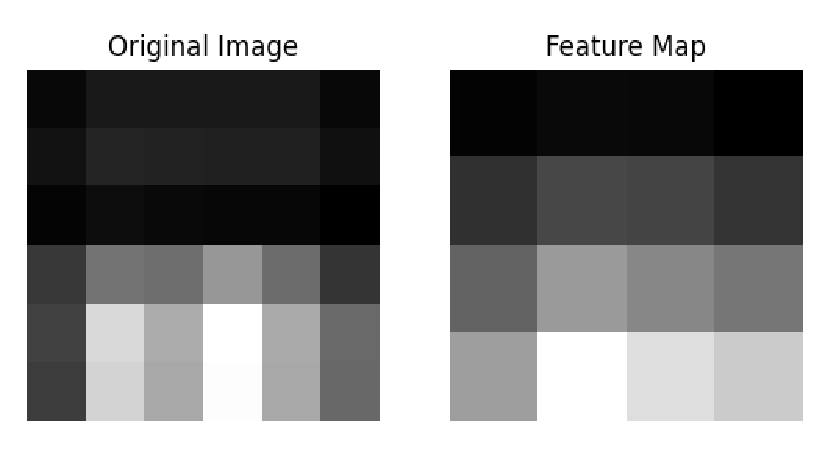
\includegraphics[width=.7\textwidth]{../Problem 11/conv_result.pdf}
	\caption{The Original Image and the Image after the convolution}
\end{figure}
\vspace{3mm}
\subsection{Question B}
Now, using the output of the convolution of the input image we are going to apply a max pooling layer with the following properties: 
\begin{itemize}
	\item $stride = \left(2,2\right)$ and 
	\item $	window\ \ shape = \left(2, 2\right)$
\end{itemize}
In general, a max pooling layer performs a downsampling operation along the spatial dimensions, width and height, of the input data. The main goal is to reduce the dimensionality of the input, which helps to control overfitting and reduces computational complexity for subsequent layers.\\
In our exercise, the size of the input matrix is reduced from $ 4 x 4 \rightarrow 2 x 2$.\\
 
The max pooling operation works by defining a spatial neighborhood, in our case a $ 2 x 2\ \ window$ and taking the maximum element from the rectified feature map within the window. This window is slid over the input data with a certain stride to produce a new matrix where each element is the maximum of a neighborhood from the input. This process effectively reduces the spatial dimensions of the feature map.\\

The result of the max pooling layer is a $2 x 2$ matrix of the same image
\begin{equation}
	max\_pooling = \begin{bmatrix}
		566 & 552   \\
		1488 & 1320 &  \\
	\end{bmatrix}
\end{equation}
\\
We can conclude that the max pooling operation only reduces the size of the feature map while preserving the most important and prominent features. It gives a more abstract and compressed representation of the input image.
\vspace{3mm}

\subsection{Question C}
As we have seen in the previous questions, the use of kernels, also known as filters, is a fundamental tool for image processing. They are essential for the efficient extraction of different features, the reduction of the number of parameters and optimal processing. In this exercise, we will emphasize the importance of kernels for extracting different features from the same input image.\\

So, for the input image (Matrix~\ref{tab:input_image}) we have the following results:
\begin{itemize}
	\item \underline{Filter $F1$}\\
	
	\begin{equation}
		F1 = \begin{bmatrix}
			-10 & -10 & -10   \\
			  5 &  5 &  5   \\
			-10 & -10 & -10   \\
		\end{bmatrix}
	\end{equation}
	\vspace{2mm}
	
	We can conclude that this filter is a type of edge detection filter, specifically designed to detect edges running horizontally in an image. \\
	In more detail, the negative values on the top and bottom rows will respond strongly to intensity changes in those directions, while the positive values in the middle row will respond to the opposite. Areas with strong horizontal edges will result in high absolute values in the convolved feature map. This means that this filter will highlight areas of the image where there is a strong intensity change from dark to light or light to dark in a horizontal direction, effectively detecting horizontal edges. To be precise, the positive values in the middle row of the kernel will align with the lighter part of a horizontal edge, while the negative values will align with the darker part.\\
	
	After applying the kernel $F1$ to our input image I, we obtain the following matrix:

	\begin{equation}
		I\_F1 = \begin{bmatrix}
			-925 & -1040 & -1000 & -845 \\
			 -3900 & -4895 & -4825 & -4160  \\
			-3750 & -5120 &-4650 & -4210   \\
			-5200 & -6990 & -6750 & -5920 \\
			\end{bmatrix}
	\end{equation}
	\vspace{2mm}
	
	As we can observe, the size of the matrix is reduced, due to the "valid" mode in the convolution operation on our code, as it only computes the convolution where the kernel fits entirely within the image boundaries.\\
	
	The values in this feature map represent the strength and location of horizontal edges detected in the input image. High absolute values, whether positive or negative, indicate strong edges, while values close to zero indicate regions with little or no horizontal edge presence.\\
	In this case, the large negative values indicate strong horizontal edges where there is a transition from light to dark pixels. This is consistent with the design of the kernel, which is tailored to detect such features in the image.
	
	
	To understand the topic, i will provide a graphical explanation.
	\begin{figure}[H]
		\centering
		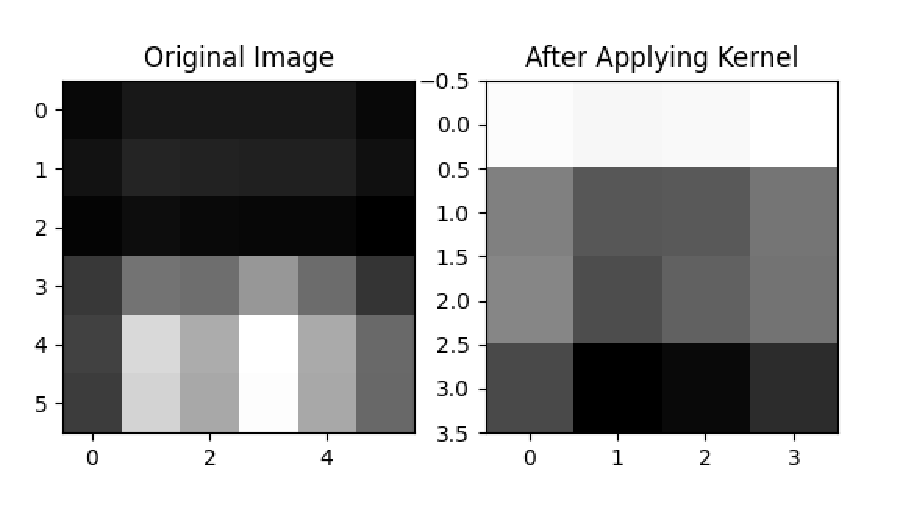
\includegraphics[width=.7\textwidth]{../Problem 11/kernel_F1.pdf}
		\caption{Before and After of the input image}
		\label{fig:kernel1}
	\end{figure}
	\vspace{3mm}
	
	\item \underline{Filter $F2$}\\
	
	\begin{equation}
		F2 = \begin{bmatrix}
			2 & 2 & 2   \\
			2 & -12 & 2   \\
			2 & 2 & 2   \\
		\end{bmatrix}
	\end{equation}
	\vspace{2mm}
	
	The filter $F2$ is a $3 x 3$ matrix with a negative value in the center and positive values surrounding it. This type of kernel is often used for edge detection, most likely to highlight the edges of objects in the image.\\
	
	This configuration indicates that the kernel is likely designed to detect points in the image where there is a central pixel that is significantly different from its surrounding pixels. Exemplifying, when this kernel is convoluted with an image, it computes a difference between the center pixel and its neighbors. If the image has a region where pixel intensity changes rapidly, the convolution operation will yield a high absolute value. In contrast, in regions of the image where pixel intensity changes slowly, the convolution operation will yield values close to zero.\\
	
	To have a better understanding, we will apply this kernel to our image I.\\
	After applying the kernel $F2$ to our image, the result is:
	
		\begin{equation}
		I\_F2 = \begin{bmatrix}
			-102 & -12 &  -4 & -86 \\
			 616  & 880 &  876 &  716  \\
			-24 & 570 & -74 & 236   \\
			-592 & 888 & -384 & 384 \\
		\end{bmatrix}
	\end{equation}
	\vspace{2mm}
	
	That being said, the positive and negative values in the feature map correspond to areas where this contrast is detected. Particularly, positive values indicate regions where the central pixel is much darker than its surroundings and negative values indicate regions where the central pixel is not significally different from its surroundings as in regions with higher positive values.\\
	
	We can figure it out by providing also this figure:
	\begin{figure}[H]
		\centering
		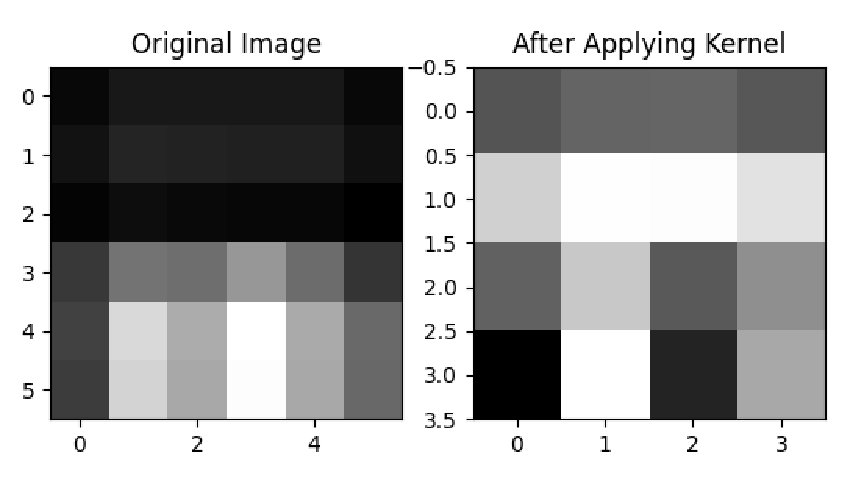
\includegraphics[width=.7\textwidth]{../Problem 11/kernel_F2.pdf}
		\caption{Before and After of the input image}
		\label{fig:kernel2}
	\end{figure}
	\vspace{3mm}
	
	The visualization in the image seems to reflect the application of such a kernel, because areas of the original image that had a central pixel with lower intensity compared to the neighbors would stand out as brighter spots in the resulting image.\\
	
	To sum up, this kind of kernel is useful for detecting features such as sharp edges, corners, or small isolated features where there is a notable contrast between a central point and its neighboring pixels. The high values (both positive and negative) in the feature map highlight these contrasting areas in the image.
	\vspace{3mm}
	
	\item \underline{Filter $F3$}\\
	
	\begin{equation}
		F3 = \begin{bmatrix}
			-20 & -10 & 0 & 5 & 10   \\
			-10 & 0 & 5 & 10 & 5  \\
			 0 & 5 & 10 & 5 & 0   \\
			 5 & 10 & 5 & 0 & -10 \\
			10 & 5 & 0 & -10 & -20\\
		\end{bmatrix}
	\end{equation}
	\vspace{2mm}
	
	We can presume that this kernel appears to be a type of edge detection filter, specifically designed to detect diagonal edges in an image.\\
	
	To elaborate, the negative values in the top-left and bottom-right corners will respond strongly to intensity changes in those directions, while the positive values in the top-right and bottom0left corners will respond to the opposite. This means that this filter will highlight areas of the image where there is a strong intensity change from dark to light or light to dark in diagonal direction, effectively detecting diagonal edges.\\
	
	By applying the kernel to our image (Matrix~\ref{tab:input_image}) we get a $2 x 2$ feature map:
	\begin{equation}
		I\_F3 = \begin{bmatrix}
			-2405 & 1000 \\
			-120 & 3915  \\
		\end{bmatrix}
	\end{equation}
	\vspace{2mm}
	
	The negative values on the left and top, transitioning to positive values on the right and bottom, indicate that this kernel might be sensitive to edges that go from dark to light in both vertical and horizontal directions.\\
	
	Graphically, this can be shown by the following figure:
		\begin{figure}[h]
		\centering
		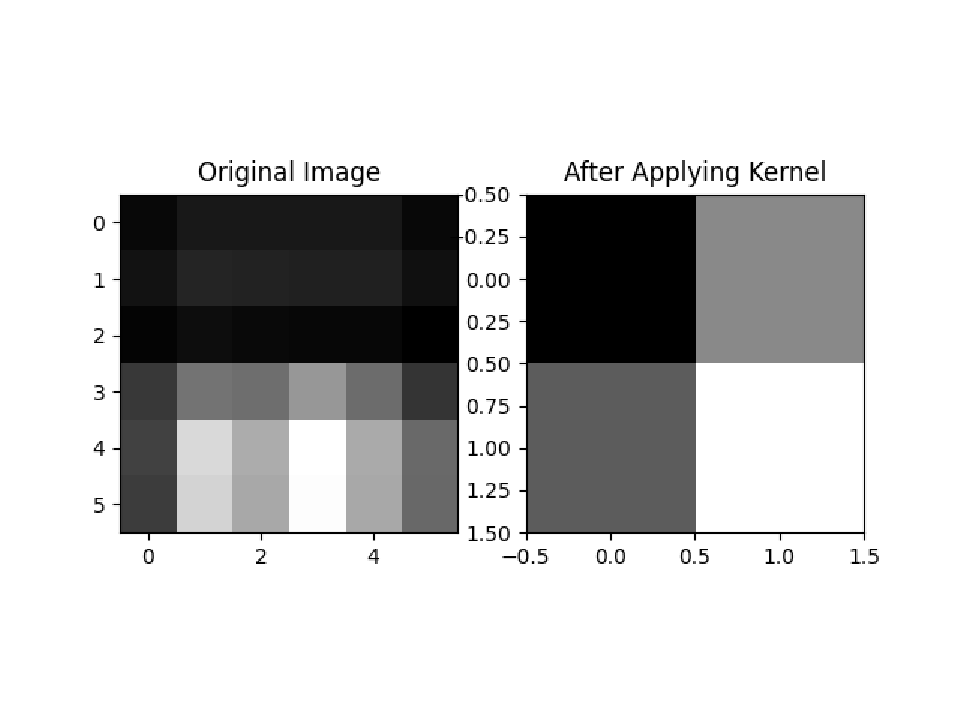
\includegraphics[width=.7\textwidth]{../Problem 11/kernel_F3.pdf}
		\caption{Before and After of the input image}
		\label{fig:kernel3}
	\end{figure}
	\vspace{3mm}
		
\end{itemize}
\vspace{5mm}







	% !TeX spellcheck = en_US
\section{Problem 12}

To compute the number of weights and biases for each convolutional layer, we need to take into consideration the size of kernels and the number of input/output channels for each layer.

\subsection{First hidden layer}
For the first hidden layer we have:
\begin{itemize}
	\item \textbf{Input Channels:} 3
	\item \textbf{Kernel Size:} 3
	\item \textbf{Output Channels:} 4
\end{itemize}

Each filter in a convolutional layer has a weight for each entry in the kernel in the kernel for each input channel, and there is one bias per filter.\\ 

The number of weights for a single filter in the first layer is the kernel size multiplied by the number of input channels:
\[
\textit{Weights per filter} = \textit{Kernel size} \times \textit{input channels} = 3 \times 3 = 9
\] \\ 

Since there are $4$ filters, the total number of weights for the first layer is: 
\[
\textit{Total weights} = \textit{Weights per filter} \times \textit{Filters} = 9\times 4 = 36.
\] \\ 

There's only one bias per filter, so the total number of biases is $4$.

\subsection{Second hidden layer}
For the second hidden layer we have:
\begin{itemize}
	\item \textbf{Input Channels:} 4 (\textit{\small from the previous layer})
	\item \textbf{Kernel Size:} 5
	\item \textbf{Output Channels:} 10
\end{itemize}

The number of weights for a single filter in the second layer is the kernel size multiplied by the number of input channels from the first layer:
\[
\textit{Weights per filter} = \textit{Kernel size} \times \textit{Input channels from previous layer} = 5 \times 4=20
\]
Since there are 10 filters, the total number of filters on the second layer is $20 \times 10 = 200$.

As far as the biases are concerned, there's only one bias per filter, so for $10$ filters, the total number is $10$.\\

Summarizing, for the two convolutional layers, we need a total of \underline{$36$ weights and $4$ biases for the first layer} and \underline{$200$ weights and $10$ biases for the second layer}.
	% !TeX spellcheck = en_US
\section{Problem 13}
Max-pooling is a process used for downsapling the input or reducing its dimensionality. It works by sliding a window across the input and taking the maximum value within that window as an output.

\subsection{Question A}
Max pooling can be accomplished using ReLU operations and in this Question we will show it and we will express $\max(a,b)$ by using them.\\

To begin with, ReLU, as we have mentioned before, is an activation function that:
\begin{itemize}
	\item For inputs $x$ where $x > 0$, the output is $x$.
	\item For inputs $x$ where $x \leq 0$, the output is $0$
\end{itemize}

Mathematically it is defined as: $\operatorname{ReLU}(x)=\operatorname*{max}(x,0)$\\

Taking this into account, to express the $\max(a,b)$ by using only ReLU operations, we can consider the following expression:\\
\begin{equation}
	max(a,b) = a \cdot ReLU(a-b) + b \cdot ReLU(b-a).
	\label{eq:problem13}
\end{equation}


Therefore, now we need to prove it: 
\begin{itemize}
	\item $\bm{For\ \ a > b:}$\\
	$a - b > 0 $ and $b - a < 0$.\\
	$\operatorname{ReLU}(a - b) = a - b$ and  $\operatorname{ReLU}(b - a) = 0$
	\vspace{1mm}
	
	By replacing these values into Equation~\ref{eq:problem13} we will have:
	
	$max(a,b) = a\cdot(a-b) + b\cdot0 = a\cdot(a-b).$
	\vspace{1mm}
	
	In this result, $a > b$, so it is the maximum value between these two and $(a - b) > 0$. Thus, the product is positive and the possible maximum.
	\vspace{1mm}
	
	Hence, the expression max(a,b) evaluates to the maximum of $a,b$.
	
	\item $\bm{For\ \ a < b:}$\\
	$a - b < 0 $ and $b - a > 0$.\\
	$\operatorname{ReLU}(a - b) = 0$ and  $\operatorname{ReLU}(b - a) = b - a$
	\vspace{1mm}
	
	By replacing these values into Equation~\ref{eq:problem13} we will have:
	
	$max(a,b) = a\cdot0 + b\cdot(b-a) = b\cdot(b-a).$
	\vspace{1mm}
	
	Similarly, $b > a$, so it is the maximum value between these two and $(b - a) > 0$. Thus, the product is positive and the possible maximum.
	\vspace{1mm}
	
	Additionally, the expression max(a,b) evaluates to the maximum of $a,b$ too.
\end{itemize}
Everything considered, we can express $\max(a,b)$ as $max(a,b) = a\cdot(a-b) + b\cdot0 = a\cdot(a-b).$
\vspace{3mm}

\subsection{Question B}



	% !TeX spellcheck = en_US
\section{Problem 14}

We are given an abstract of a CNN that classifies images into two classes. Its structure is as follows:
\begin{itemize}
	\item \textbf{Input}: $100 \times 100$ grayscale images.
	\item \textbf{Layer 1}: Convolutional layer with $100 \ 5\times 5$ convolutional filters.
	\item \textbf{Layer 2}: Convolutional layer with $100 \ 5\times 5$ convolutional filters.
	\item \textbf{Layer 3}: Max Pooling layer with reduction of $2$.
	\item \textbf{Layer 4}: Dense layer with 100 units.
	\item \textbf{Layer 5}: Dense layer with 100 units.
	\item \textbf{Layer 6}: Single output unit.
\end{itemize}

In order to calculate all the weights in this CNN, we have to consider each layer separately:\\

\begin{minipage}[l]{0.47\textwidth}
	\textbf{Layer 1:}
	\begin{itemize}
		\item Input size: $100 \times 100$.
		\item Filter size: $5 \times 5$.
		\item Number of filters: $100$.
		\item Weights: Each filter has $5 \times 5$ weights and there's a bias per filter.
		\begin{itemize}
			\item Weights per filter: $5 \times 5=25$.
			\item Total weights: $25\times 100=2500$.
			\item Total biases: $100$ (1 per filter).
		\end{itemize}
	\end{itemize}
	So, this layer produces shape $\left(96,96,100\right)$ and in total we have $2500 + 100 = 2600$ weights. \\ {\small Output shape is calculated as: input num $ - $ kernel size $+ 1$}
\end{minipage}
\hfil
\begin{minipage}[r]{0.47\textwidth}
	\textbf{Layer 2:}
	\begin{itemize}
		\item Input channels: $100$ (from layer 1).
		\item Filter size: $5 \times 5$.
		\item Number of filters: $100$.
		\item Weights: Each filter has $5 \times 5$ weights for each input channel.
		\begin{itemize}
			\item Weights per filter: $5 \times 5 \times 100 = 2500$.
			\item Total weights: $2500\times 100 = \num{250000}$.
			\item Total biases: $100$ (1 per filter).
		\end{itemize}
	\end{itemize}
	In total, we have $\num{250000} + 100 = \num{250100}$ weights and it creates an output shape of $\left(92,92,100\right)$.
\end{minipage}

\vspace{3mm}

Moving on to \textbf{Layer 3}, it's important to note that this layer doesn't have any weights or biases because it's a pooling layer. Pooling layers downsample the output from the previous layer.
In this case, Layer's 2 output is reduces to $46 \times 46 \times 100$  from $92 \times 92 \times 100$.\\

\textbf{Layer 4} is a dense (\textit{fully connected}) layer with an input that of the max pool layer. Before it connects with the max pool layer, the data must be converted from multi-dimensional array into a one-dimensional array.
After this is done, the input data of layer 4 have a size of $46 \times 46 \times 100 = \num{211600}$. So, in order to calculate the weights and biases, we only need two information: the number of neurons ($100$) and the number of neurons of the previous layer ($\num{211600}$).\\
The equation for total weights of this layer is: \\
$\textit{number of neurons} \times \textit{number of neurons of the previous layer} + \textit{number of neurons} = 100 \times 211600 + 100 = 21160100$. \\ 

\textbf{Layer 5} is also a dense layer and the procedure for calculating the weights is the same as above. 
We have $100$ units in this layer and $100$ in the last one, so total weights are: $100 \times 100 + 100 = \num{10100}$. \\

Moving on to the \textbf{output layer}, weights are equal to the input units and bias is only $1$, so this layer's weights number is $100 +1 = 101$. \\ 

The total number of weights is:
\[
\begin{gathered}
\text{Total Weights} = \text{Layer 1} + \text{Layer 2} + \text{Layer 3} + \text{Layer 4} + \text{Layer 5} + \text{Layer 6} = \\
= \num{2600} + \num{250100} + \num{21160100} + \num{10100} + \num{101} = \\  =\mathbf{\num{21423001}} \text{ weights}
\end{gathered}
\]
\vspace{3mm}
	
	
	
\end{document}